\documentclass[a4paper,11pt,openright,oneside]{book}
\frenchspacing

\usepackage[utf8]{inputenc}
\usepackage[italian]{babel}
\usepackage[dvips]{graphicx}
\usepackage{url}
\usepackage{rotating}
\usepackage{verbatim}
\usepackage{longtable}
\usepackage[boxed]{algorithm2e}
\usepackage{amsmath}

\usepackage{amssymb} %simboli matematici
\usepackage{latexsym} %?
\usepackage{mathrsfs} %?
\usepackage{amsfonts}

\usepackage{hyperref}

\usepackage{frontespizio}
\usepackage{listings} %Per inserire codice
\usepackage[usenames]{color}%Per permettere la colorazione dei caratteri 
\usepackage{fancyhdr} 


\usepackage{listings} %Per inserire codice
\usepackage[usenames]{color}%Per permettere la colorazione dei caratteri 

\usepackage{titlesec,blindtext}
\usepackage[Lenny]{fncychap}

\usepackage{eso-pic}
\newcommand\BackgroundPicture{
   \put(0,0){
     \parbox[b][\paperheight]{\paperwidth}{
       \vfill
       \centering
       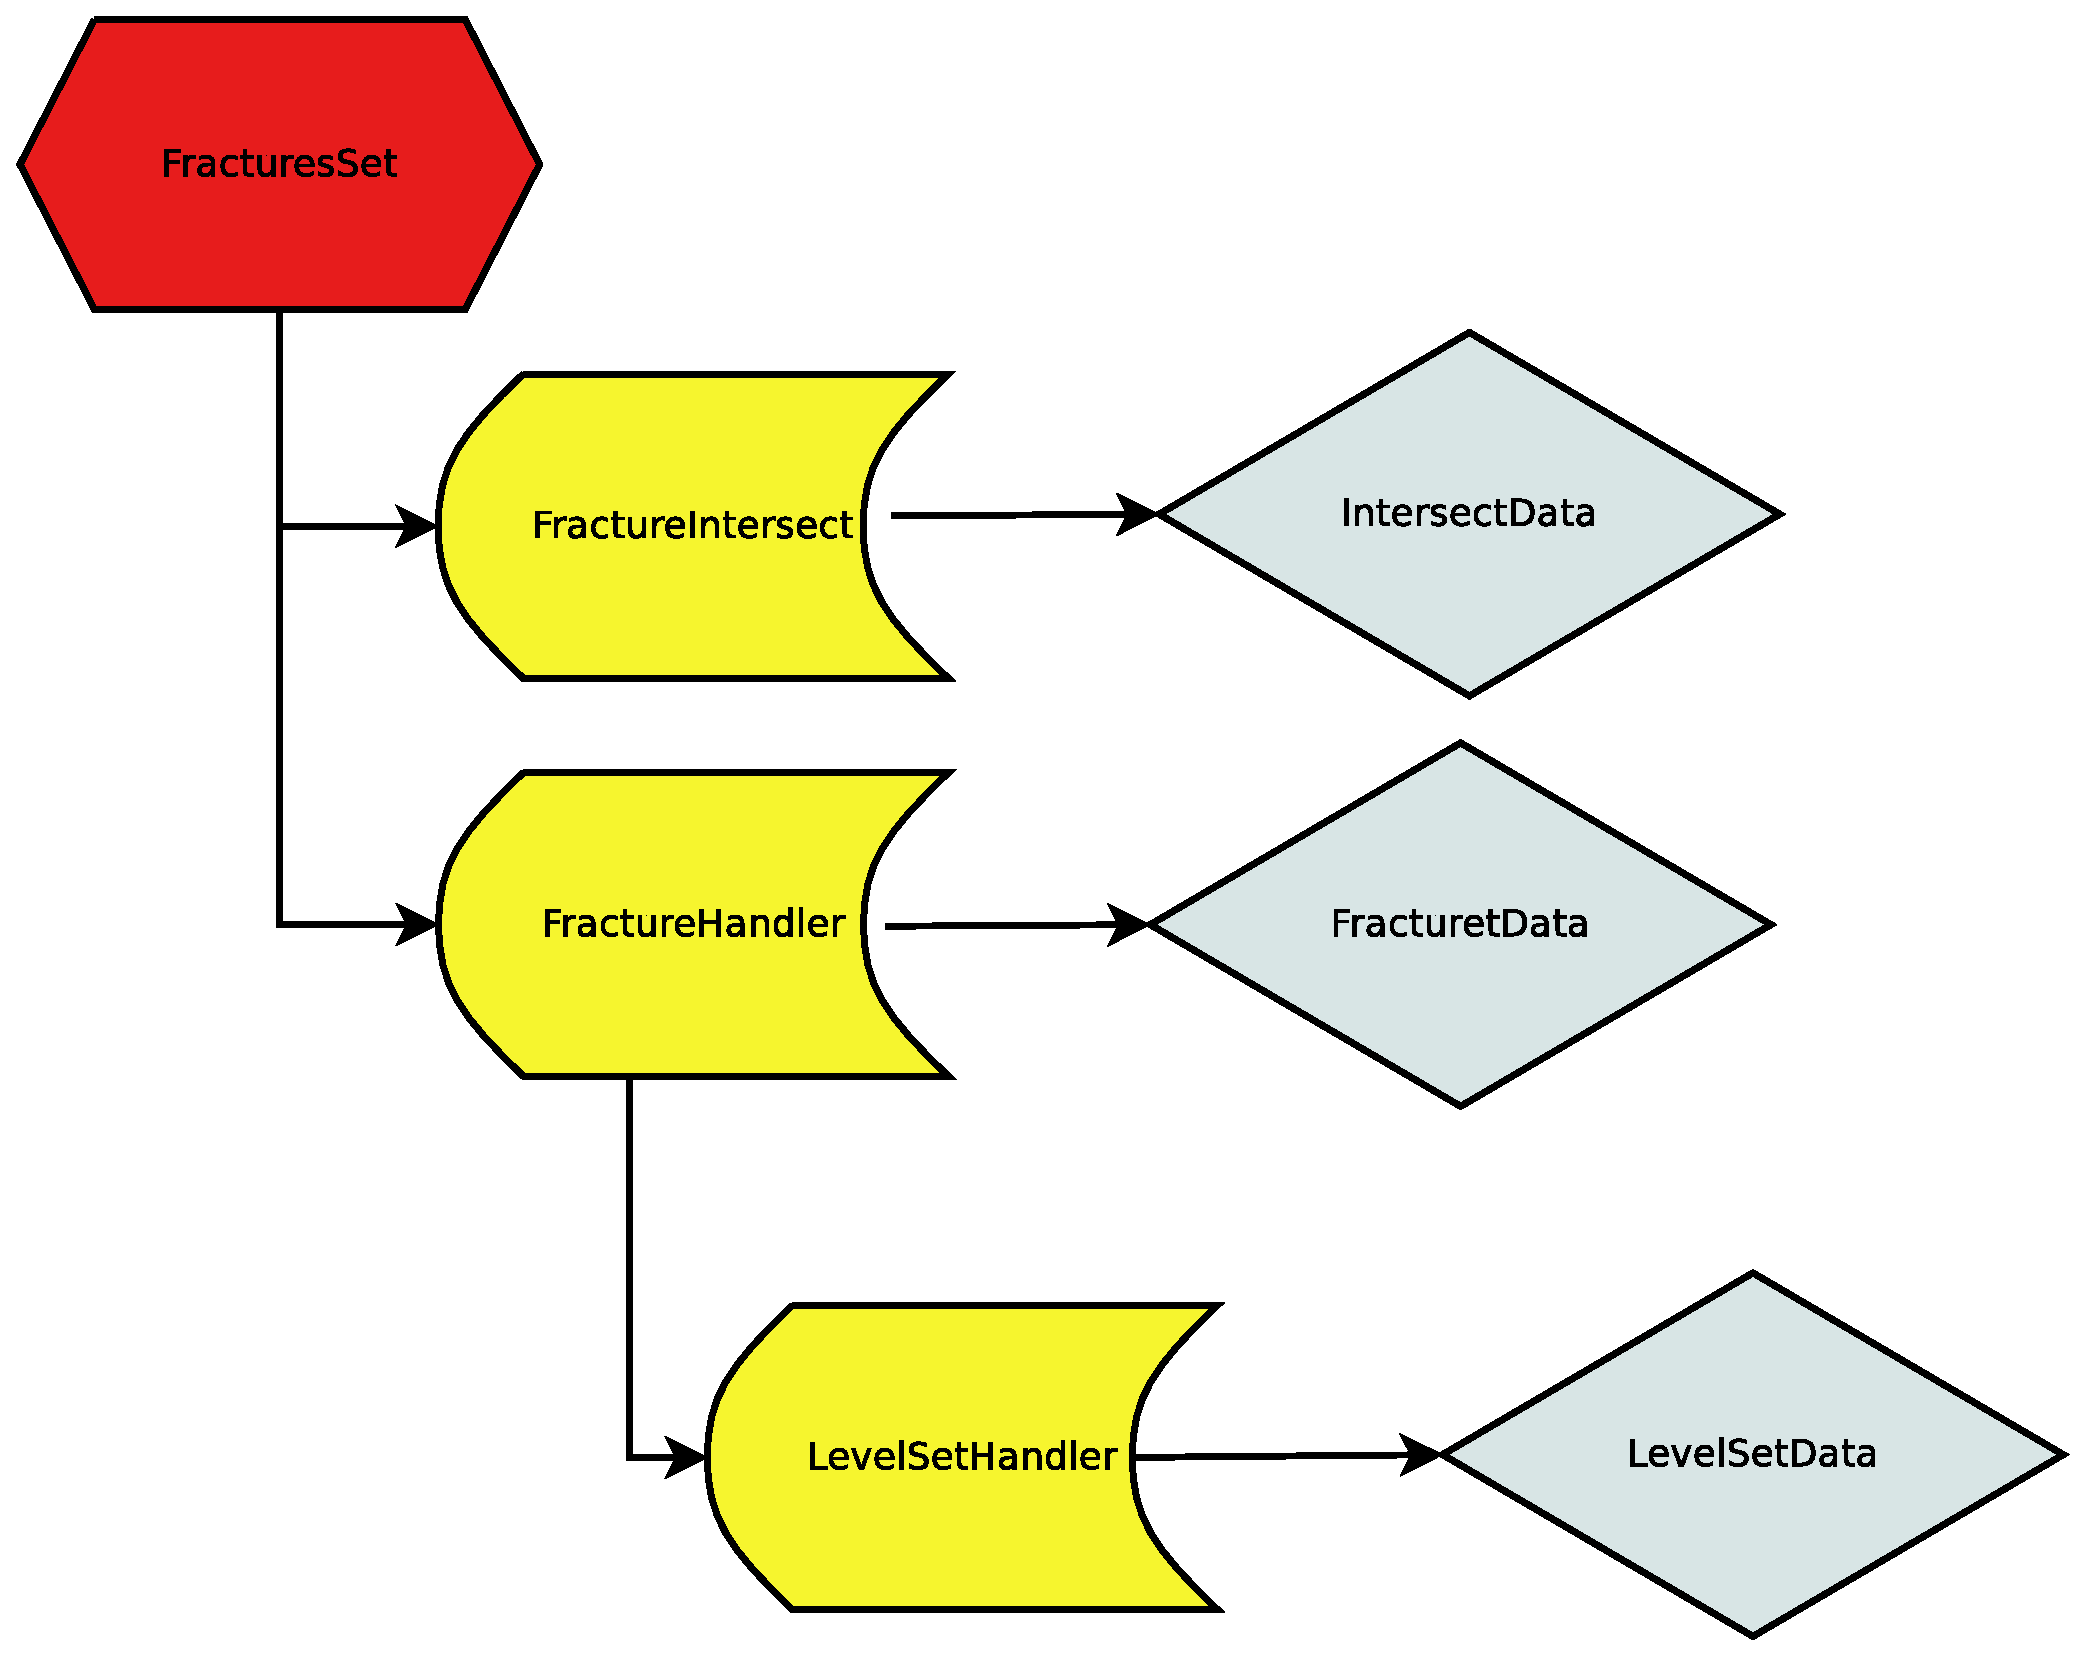
\includegraphics[width=\textwidth]{img/fratture.eps}
       \vfill
     }}}



%\usepackage[Sonny]{fncychap}
%\usepackage[toc]{glossaries}
%\makeglossaries
%\usepackage{lscape}

\ChNameVar{\fontsize{14}{16}\usefont{T1}{phv}{m}{n}\selectfont}
\ChNumVar{\fontsize{60}{62}\usefont{T1}{ptm}{m}{n}\selectfont}

 
\begin{document}

\begin{frontespizio}

\Istituzione{POLITECNICO DI MILANO}
\Logo{logo_polimi}
\Facolta{Ingegneria Industriale e dell'informazione}
\Corso[Laurea]{Ingegneria Matematica}
\Annoaccademico{2013-2014}
\Sottotitolo{Imposizione delle condizioni d'interfaccia per intersezioni di tipo Biforcazione}
\Titolo{\color[rgb]{.6,0,0} Soluzione del problema di Darcy in un network di fratture}
\Candidato[]{Claudia Bonomi matr. 804378}
\Candidato[]{Maria Iemoli matr. 800499}
\Titoletto{Progetto per il corso di Programmazione Avanzata per il Calcolo Scientifico}
\Relatore{ Luca Formaggia}
\Relatore{ Anna Scotti}
\Rientro{1cm}
\Margini{1.5cm}{2cm}{1.5cm}{3cm}
\end{frontespizio} 


\hypersetup{
    %colorlinks,
    citecolor=black,
    filecolor=black,
    linkcolor=black,
    urlcolor=black
}


%\maketitle

%\hyphenation{net-list}\pagestyle{empty}
%
\usepackage[latin1]{inputenc}
\usepackage[italian]{babel}
\usepackage{latexsym}
\usepackage{epsfig}
\usepackage{tabularx}
\usepackage{morefloats}
\usepackage{setspace} 
\usepackage{url}
\usepackage[sans,nouppercase]{frontespizio}



%\begin{document}
\begin{frontespizio}
\Universita{Politecnico di Milano}
\Logo{logo_polimi}
\Facolta{Scuola di Ingegneria Industriale e dell'Informazione}
\Corso{Ingegneria Matematica}
\Annoaccademico{2013--2014}
\Titoletto{Progetto per il corso di ANEDPII}
\Titolo{Segmentazione del Ventricolo Sinistro con tecniche GAC}
\Candidato[800499]{Maria Iemoli}
\Relatore{Simona Perotto}
\Relatore{Elena Faggiano}
\end{frontespizio}



%\newpage
\chapter*{Introduzione}

Il presente progetto si inserisce nell'ambito dello studio del moto di un fluido in un mezzo poroso.\cite{habilitationsschrift}
Lo scopo è quello di studiare e risolvere il problema nel caso di un network di fratture che si intersecano. \\
Il nostro progetto parte da un codice già esistente in C++ in grado di risolvere il problema di Darcy nel caso in cui due fratture abbiano un'intersezione a \textit{X}. \cite{ESAIM}
Il nostro obiettivo è quello di estendere il codice ad altri tipi di intersezione, in particolare vogliamo risolvere il problema in presenza di tre fratture che si intersecano in un unico punto comune formando una \textit{Y}.\\
Per l'implementazione e la risoluzione del problema tramite elementi finiti, abbiamo utilizzato principalmente la libreria \texttt{GetFEM++}, un insieme di liberie scritte in C++ che mettono a disposizione dell'utente una serie di funzioni utilizzabili per la soluzione dei problemi FEM. \\
La nostra implementazione si basa su un modello ridotto, considera cioè le fratture come delle grandezze 1d, trascurandone lo spessore. Per poter ricavare le condizioni d'interfaccia nel caso della nuova intersezione si è reso necessario ritornare al modello 2d, e quindi considerare l'intersezione come un triangolo e non come un punto \cite{Paper} \cite{LDAP}.

\pagestyle{plain}
\pagenumbering{Roman}
\include{prefazione}

\pagenumbering{arabic}
\tableofcontents

\chapter{Mezzi porosi e legge di Darcy}

I materiali porosi sono dei mezzi in cui si possono distinguere due costituenti: una matrice solida, la parte che costituisce la struttura rigida del corpo, e lo spazio vuoto restante, che può essere riempito con uno o più fluidi. \\
Risulta spesso interessante studiare il moto di un fluido in un mezzo poroso in cui sia possibile distinguere delle fratture o dei canali al suo interno. Nell'analisi del moto di un fluido in una frattura tra diversi strati geologici, ad esempio,  si può pensare che il fluido, oltre a insinuarsi e scorrere nella frattura, si propaghi mediante filtrazione negli strati adiacenti la frattura stessa.
Un'altra possibile applicazione in ambito idrogeologico riguarda lo studio di come i fiumi irrighino il terreno ad essi circostante. 
\par Il moto del fluido all'interno del mezzo poroso viene descritto tramite la legge di Darcy.  Generalmente le dimensioni delle fratture sono di molto inferiori a quelle del dominio occupato dal mezzo poroso. Questo ha portato allo sviluppo di tecniche per lo studio del flusso all'interno delle fratture basate su modelli ridotti. Questi modelli si inseriscono nella categoria dei modelli multiscala, ed hanno il vantaggio di evitare la risoluzione del campo di moto sulle scale spaziali molto piccole nella frattura.

\section{Legge di Darcy}
La legge di Darcy descrive la filtrazione di un fluido incomprimibile all'interno di un mezzo poroso. In particolare costituisce un legame tra il campo di velocità del fluido e il gradiente di pressione nel mezzo poroso. \\
Il moto di un fluido incomprimibile in un mezzo poroso ( considerando z=0 come quota di riferimento) può essere descritto dalla seguente coppia di equazioni:
 
\begin{equation}
\textbf{u} =- \frac{\textbf{K}}{\mu}\nabla {p} \footnote{Più avanti indicheremo $\frac{\textbf{K}}{\mu}$ con $\textbf{K}$ per semplicità}
\end{equation}\label{Darcy}

\begin{equation}
\nabla \cdot u =f
\end{equation}

dove:
\begin{enumerate}
\item[-] \textbf{u}(\textbf{x}, t) è il campo di velocità macroscopica del fluido misurata in [\textit{m/s}];
\item[-] \textbf{K}(\textbf{x}) è il tensore simmetrico di permeabilità assoluta misurato in [\textit{m$^2$}];
\item[-] \textit{p}(\textit{x,t}) è la pressione del fluido in [\textit{Pa}]=[\textit{N/m$^2$}];
\item[-] \textit{$\mu$} (\textbf{x}, t) rappresenta la viscosità dinamica del fluido in [\textit{Pa s}], che per semplicità verrà considerata costante;
\item[-] \textit{f}(\textbf{x}, t) rappresenta il termine sorgente di dimensione [\textit{s}$^{-1}$].
\end{enumerate}


La prima equazione è la legge di Darcy e deriva dalla conservazione del momento nelle equazioni di Navier-Stokes con opportuni passaggi, mentre la seconda rappresenta la conservazione della massa. \\
L'approssimazione con il modello di Darcy è valida per fluidi Newtoniani con bassi valori del numero di \textit{Raynolds} ($Re<10$), per cui gli effetti inerziali possono essere trascurati. Per valori maggiori è necessario estendere il modello poichè l'equazione \ref{Darcy} presenta dei limiti.


 \section{Formulazione debole del problema}
Il problema del flusso di un fluido in un mezzo poroso assume la seguente forma:

\begin{equation}
\begin{cases}
\textbf{K}^{-1}  \textbf{u} +\nabla {p} =0 \\
\nabla  \cdot u =f
\end{cases} 
\end{equation}\label{sistema}

\noindent con condizioni al contorno:

\begin{equation}
\begin{cases}
\textbf{u} \cdot \textbf{n}_{\Omega} =0  & su \;  \Gamma ^u\\
p =g & su \; \Gamma ^p
\end{cases}
\end{equation}\label{bc}

Per ricavare la formulazione debole del problema, così da poter discretizzare con gli elementi finiti, moltiplichiamo la prima equazione del sistema \ref{sistema} per una funzione test \textbf{v}, la seconda per una funzione test \textit{q} e integriamo su $\Omega$. \\
La formulazione debole diventa: trovare (\textbf{u}, $p$) tali che:
\begin{equation}
\begin{split}
\int_{\Omega} (\textbf{K}^{-1} \textbf{u}) \cdot \textbf{v} \, dx  - \int_{\Omega} p \nabla \cdot \textbf{v} \, dx  + \int_{\Gamma^p} g \, \textbf{u} \cdot \textbf{n} \, d\Gamma = 0 & \quad  \forall \, \textbf{v} \in \textbf{W} \\
\int_{\Omega} \nabla \cdot \textbf{u} q \, dx = \int_{\Omega} f q \, dx & \quad \forall \, q \in Q
\end{split}
\end{equation}\label{formdebole}

dove: 

\begin{equation*}
\begin{split}
\textbf{W} &=H_{div}(\Omega) = \left \{ \textbf{w}\in [L^2(\Omega)]^2, \nabla \cdot \textbf{w} \in L^2(\Omega), \textbf{v} \cdot \textbf{n} = 0 \, su \, \Gamma^n \right \} \\
Q &= L^2(\Omega) 
\end{split}
\end{equation*}

Per la discretizzazione in spazio scegliamo lo spazio degli elementi finiti di grado due per la velocità e uno per la pressione e ricaviamo la seguente formulazione algebrica:
\begin{equation}
\begin{cases}
A11 \textbf{U} \, +A12 \textbf{P} = F_1 \\
A12^T \textbf{U} = F_2
\end{cases}
\end{equation}


dove $ A11 \in \mathbb{R}^{N_u \times N_u}$ e $A12 \in \mathbb{R}^{N_p}$  sono le matrici realative alle forme bilineari $a(\cdot, \cdot)$ e $b(\cdot, \cdot)$ definite come:

$$ a(\textbf{u}_h , \textbf{v}_h)= \int_{\Omega} (\textbf{K}^{-1} \textbf{u}_h) \cdot \textbf{v}_h \, dx \qquad b(\textbf{u}_h, q) = - \int_{\Omega} q_h \nabla \cdot \textbf{u}_h \, dx  $$
$$ f1(\textbf{u}_h) = \int_{\Gamma^p} g_h \, \textbf{u}_h \cdot \textbf{n} \, d\Gamma \qquad f2(q_h) =  - \int_{\Omega} f q \, dx $$

Nel nostro caso quindi, per risolvere il flusso di un fluido all'interno di una frattura in un mezzo poroso si ottiene il seguente sistema algebrico:
\begin{equation}
\left[\begin{matrix}A_{11} &A_{12} \\A_{12}^T & 0 \end{matrix}\right] \, \left[\begin{matrix}U  \\P \end{matrix}\right] = \left[\begin{matrix}F_{1} \\F_{2} \end{matrix}\right] 
\end{equation}
\label{sistemaAlgebrico}

Se vi sono più fratture che si intersecano è necessario imporre delle condizioni che leghino i rispettivi flussi e le rispettive pressioni. Il codice da cui siamo partite impone le condizioni d'interfaccia nel caso di un'intersezione di tipo \textit{Cross} in modo debole. Il nostro codice, come verrà spiegato più avanti, impone le condizioni d'interfaccia nel caso della \textit{Biforcazione} in maniera forte, ossia una volta che il sistema algebrico è già stato assemblato.
\lstnewenvironment{Code03_01}[1][]{ \lstset{showspaces=false, showtabs=false,tabsize=2,basicstyle=\small\ttfamily, columns=fullflexible,framexrightmargin=+.1\textwidth, keywordstyle=\color{red}\bfseries, commentstyle=\color{blue},language=C++, basicstyle=\small,  numberstyle=\tiny, stepnumber=1, numbersep=5pt, frame=shadowbox, #1}}{}


\chapter{Considerazioni preliminari}

\section{Strumenti di sviluppo}
Lo sviluppo del nostro progetto ha richiesto l'uso di strumenti specifici atti a facilitare e sistematizzare la gestione del codice quali \texttt{git}, \texttt{CMake} e \texttt{Dxygen}.\\

\subsection{\texttt{Git}}
\href{https://github.com/}{\texttt{Git}} è un sistema di controllo versione utilizzabile direttamente da linea di comando, molto diffuso è utile per tenere traccia delle varie fasi di sviluppo del codice. Git gestisce in modo adeguato i contributi al codice provenienti da agenti esterni e permette la condivisione del codice.\\
Il codice del progetto è reperibile su \texttt{git} ed è possibile scaricarlo e collabolare allo sviluppo clonando il codice dalla repository  \href{https://github.com/}{\texttt{GitHub}}:\\
\begin{center}
\texttt{ git clone https://github.com/mariaiemoli/progetto.git}
\end{center}
Nella cartella principale è contenuto anche un file \texttt{.gitignore}, in cui sono specificate le estensioni dei files e le sottocartelle che non devono essere visionati in una repository \texttt{git}. In particolare non si è interessati ai files temporanei che vengono eventualmente generati dagli editor, e alle cartelle generate da uno scorretta configurazione di \texttt{Doxygen}.

\subsection{\texttt{CMake}}
\href{http://www.cmake.org/}{\texttt{CMake}} è un software libero multipiattaforma nato per l'automazione dello sviluppo. Sostanzialmente con l'uso di \texttt{CMake} è possibile configurare e generare Makefile per il sistema operativo in uso. Questo facilita la diffusione del codice tra sviluppatori, non dovendo far altro che lanciare \texttt{CMake} e lasciare che sia lui ad occuparsi della ricerca di compilatori e librerie locali e della costruzione di software.\\
\texttt{CMake} si basa sulla creazione di files \texttt{CMakeLists.txt} nella directory del progetto, che contengono le direttive necessarie per creare il \texttt{Makefile} per compilare ed eseguire il codice. \\
Nella directory principale si trova un primo file \texttt{CMakeLists.txt} in cui si impostano i parametri fondamentali quali la dipendenza dalla versione di \texttt{CMake}, il nome del progetto, si includono le directory dei sorgenti nel path di compilazione e si caricano le librerie esterne utilizzate dai sorgenti. \\
le librerie che vengono caricate sono:
\begin{enumerate}
\item[-] \texttt{Eigen}, libreria template per l'algebra lineare usata principalmente nella fase di imposizione delle condizioni di interfaccia sul triangolo di intersezione nel caso della biforcazione, per il modello ridotto;
\item[-] \texttt{Getfem++}, libreria matematica per gli elementi finiti usata per scrivere e risolvere il problema numerico;
\item[-] \texttt{Blas} (Basic Linear Algebra Subprograms) e \texttt{Qhull}, librerie necessarie per \texttt{Getfem++};
\item[-] \texttt{Doxygen}, usato per generare la documentazione
\end{enumerate}

\begin{Code03_01}
CMAKE_MINIMUM_REQUIRED( VERSION 2.8 )

PROJECT(PACS)

SET(CMAKE_CXX_FLAGS "-std=c++0x -Wall ${CMAKE_CXX_FLAGS}")

SET(CMAKE_MODULE_PATH 
	${CMAKE_SOURCE_DIR}/cmake ${CMAKE_MODULE_PATH})

# Include Eigen3
FIND_PACKAGE(PkgConfig)
PKG_CHECK_MODULES(EIGEN3 REQUIRED eigen3)
INCLUDE_DIRECTORIES(${EIGEN3_INCLUDE_DIRS})

# Include Doxygen
find_package(Doxygen)
[ ... ]

# Include Getfem
if (GETFEM_LIBRARIES AND GETFEM_INCLUDE_DIRS)
[ ... ]

#Include for BLAS library
find_package ( BLAS )
[ ... ]


#Include for LAPACK library
find_package ( LAPACK )
[ ... ]

#Include for QHULL library
set(QHULL_MAJOR_VERSION 6)
[ ... ]

SET(CMAKE_INSTALL_PREFIX 
${CMAKE_SOURCE_DIR}/install-dir CACHE PATH "" FORCE)

ADD_SUBDIRECTORY(src)
ADD_SUBDIRECTORY(test)
\end{Code03_01}

%% $

Per poter usare \texttt{CMake} è necessario posizionarsi nella directory in cui è contenuto il progetto e creare una cartella in cui compilare il codice. Per lanciare \texttt{CMake} è necessario digitare i seguenti comandi: \\ 

\par  \texttt{cd $<$build\_dir$>$ } 
\par \texttt{cmake $<$source\_dir$>$}\\

\noindent \texttt{CMake} imposta le variabili di path come definito nel file  \texttt{CMakeLists.txt}, esamina le dipendenze da librerie esterne e procede esaminando le sottocartelle aggiunte nel file di configurazione. In particolare esamina le sottocartelle \texttt{src} e \texttt{test}, in cui sono presenti altri files  \texttt{CMakeLists.txt}, che impostano i rispettivi obiettivi e definiscono le rispettive sottocartelle. Questo permette a \texttt{CMake} di esaminare tutta la directory in cui è contenuto il progetto in maniera ricorsiva. \\
%Nella cartella \texttt{src} il file  \texttt{CMakeLists.txt} aggiunge la creazione di una libreria a partire dal codice del progetto. \\
%\begin{Code03_01}
%ADD_LIBRARY(pacs ${TARGET_SRC} ${TARGET_HANDLER})
%\end{Code03_01}

\par \noindent Nella cartella test si trovano delle sottocartelle ognuna delle quali contenente un file data di esempio per poter eseguire il codice e un file  \texttt{CMakeLists.txt} . Il file  \texttt{CMakeLists.txt} nella cartella dei test definisce gli obiettivi e i collegamenti necessari per l'esecuzione. 

\par Una volta che il \texttt{Makefile} è stato generato è possibile compilare il codice con il comando: \\ 
\par \texttt{make}\\

\noindent Questo crea in ogni sottocartella della cartella \texttt{test} un eseguibile chiamato \texttt{Test}. Per poterlo eseguire è sufficiente lanciare da terminale, dopo essersi posizionati nella directory corretta, 
\par \texttt{ .\textbackslash Test-iesimo }

\subsection{\texttt{Doxygen}}
\href{www.doxygen.org/}{\texttt{Doxygen}} è un sistema multipiattaforma molto diffuso per la generazione automatica della documentazione di un codice. Per ottenere la documentazione è necessario introdurre nel codice dei commenti con una sintassi particolare, e il risultato contiene l’elenco delle classi implementate, i loro diagrammi di collaborazione e la descrizione di metodi ed attributi.
Per poter creare la documentazione al codice con \texttt{Doxygen} è necessario che nella cartella principale sia presente il file \texttt{Doxygen}, in caso contrario è necessario crearlo con il comando:\\
\par \texttt{Doxygen -g}\\

\noindent In questo file sono definite le variabili che permettono di creare la documentazione come il nome del progetto, la directory dove creare la documentazione, le cartelle dove si trovano i sorgenti e l'estensione dei files da considerare.

\begin{Code03_01}
PROJECT_NAME 				=	 Problema di Darcy in un network di fratture
OUTPUT_DIRECTORY			=	./build/doc
INPUT						= 	./src ./test
FILE_PATTERNS				= 	*.cc *.h
HAVE_DOT					=	YES
COLLABORATION_GRAPH		=	YES
HIDE_UNDOC_RELATIONS		=	NO
\end{Code03_01}

\noindent Dopo aver lanciato \texttt{CMake} è possibile generare la documentazione semplicemente eseguendo: \\
\par \texttt{cd $<$build\_dir$>$} 
\par \texttt{make doc} \\

\noindent Questo crea una sottocartella \texttt{build/doc} che contiene la documentazione \texttt{html} e \LaTeX{}.

\newpage

\section{Dati del problema}

\subsection{Intersezioni}
Come è stato precedentemente detto, il codice di partenza trattava un tipo particolare di intersezione tra fratture, da noi chiamato \textit{Cross}. Questo tipo di intersezione ha la seguente forma:

\begin{figure}[htbp]
\begin{center}
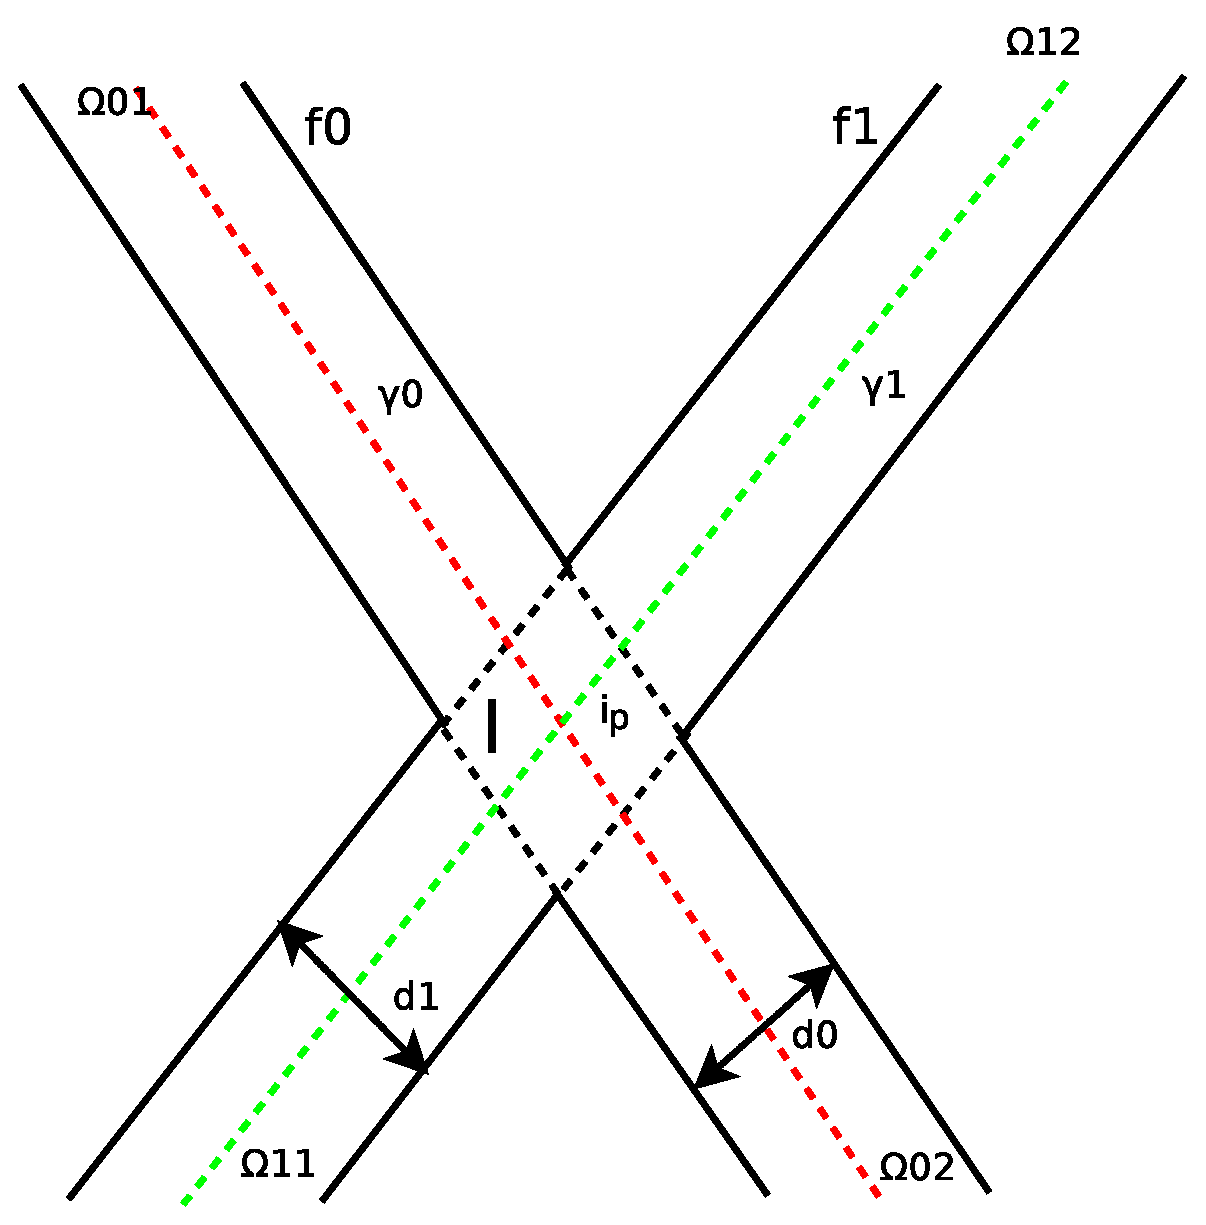
\includegraphics[width=0.4\textwidth]{img/cap2/cross.eps}
\caption{Struttura di un'intersezione di tipo \textit{Cross} tra due fratture.}\label{Cross}
\end{center}
\end{figure}

\noindent L'area di intersezione è constituita da un parallelogramma che suddivide ogni frattura in due zone $\Omega_{i1}$ e $\Omega_{i2}$. Il modello su cui noi ci basiamo riduce la frattura, qui rappresentata in un dominio $\mathbb{R}^{2}$, alla retta di sostegno $\gamma_i$. In questo modo l'intersezione si riduce ad un punto.\\
Il tipo di intersezione su cui ci siamo concentrate noi, invece, ha la seguente forma:

\begin{figure}[htbp]
\begin{center}
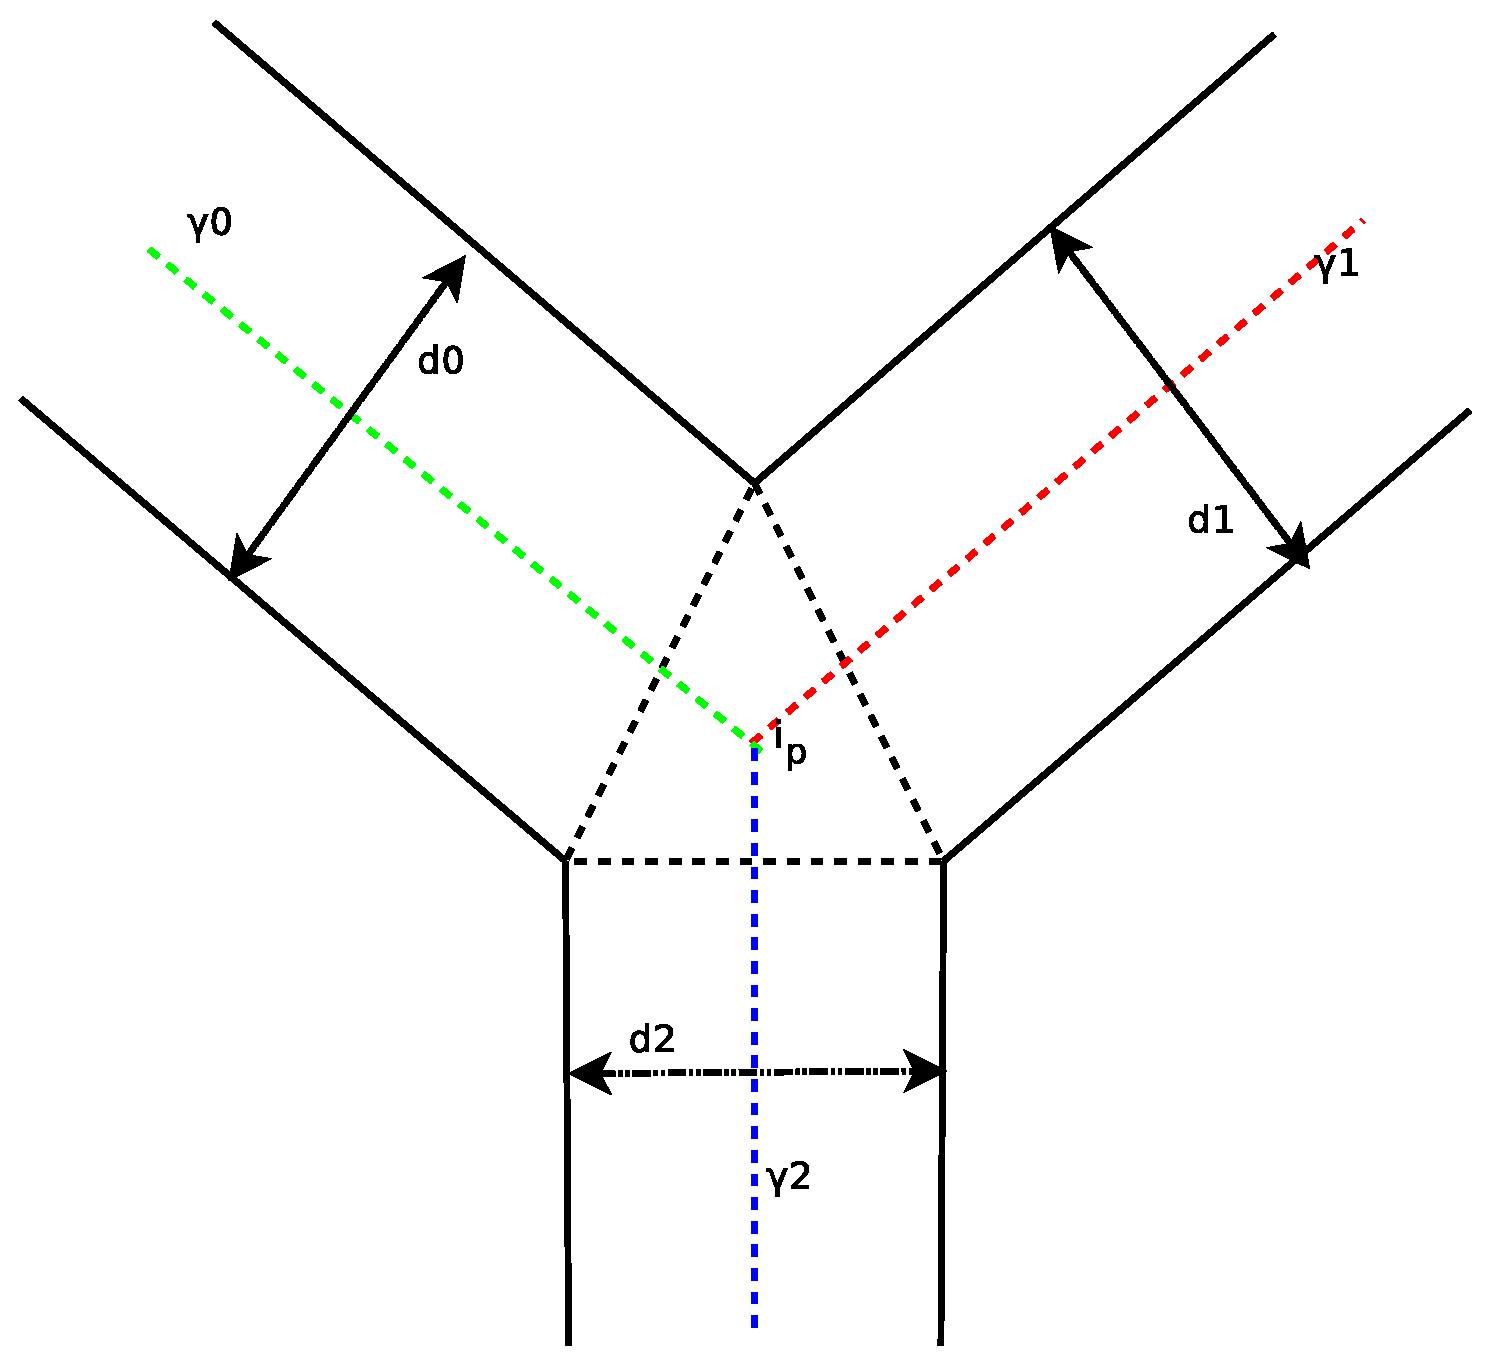
\includegraphics[width=0.4\textwidth]{img/cap2/bifurcation.eps}
\caption{Struttura di un'intersezione di tipo \textit{Bifurcation} tra due fratture.}\label{Bifurcation}
\end{center}
\end{figure}

\noindent In questo caso le fratture coinvolte sono tre e la zona interessata dall'intersezione è rappresentata da un triangolo. Anche qui consideriamo un modello ridotto e le fratture sono individuate dalle rette di sostegno $\gamma_i$ in $\mathbb{R}$. Le condizioni d'interfaccia che vengono ricavate in questo caso valgono solo nel caso in cui le tre fratture si intersechino in un unico punto comune $i_p$ e tale punto sia contenuto nel triangolo d'intersezione nella rappresentazione 2d.

\subsection{File data}

I dati per la definizione del problema sono definiti nei file .txt contenuti nella sottocartella \texttt{dati}. \\
\noindent Ognuno di questi files ha la seguente struttura:

\begin{enumerate}
\item[-] una prima parte dove vengono definite la directory dove trovare l'eventuale mesh da importare, la directory dove salvare i risultati e il numero di fratture che entrano in gioco;
\item[-] una sezione dedicata a parametri e grandezze necessari per la definizione del dominio del mezzo;
\item[-] una sezione per ogni frattura con la dichiarazione del level set, dei parametri che individuano il segmento che rappresenta la frattura e delle grandezze necessarie per risolvere il problema di Darcy.
\end{enumerate}

\begin{Code03_01}[caption={Definizione del dominio}]
meshFile = meshes/mesh		//   directory da cui importare eventualmente la mesh
folderVTK = ./vtk/				//   directory dove salvare i risultati

numberFractures = 3

[mediumData]					//   informazioni legate al mezzo poroso in questione

   [./domain]					//   informazioni necessarie per costruire o importare la mesh 
     [ ... ]
   [../]

   [./darcy]					//   informazioni sulla natura permeabile del mezzo
     invK = 1.
     invKDist11 = 1.
     invKDist12 = 0.
     invKDist22 = 1.
     [...]	
   [../]

[../]

\end{Code03_01}

\par \noindent Nonostante il nostro problema si concentri solamente sulla soluzione del flusso all'interno delle fratture, noi costruiamo comunque la mesh relativa al mezzo. Questa mesh verrà usata solamente come supporto, sarà puramente accessoria nel corso dell'implementazione. \\
 \noindent Per quanto riguarda la permeabilità, poichè le fratture sono costituite dallo stesso materiale, questa resta uguale in tutto il dominio, sia nel mezzo che nelle fratture. 

\begin{figure}[htbp]
\begin{center}
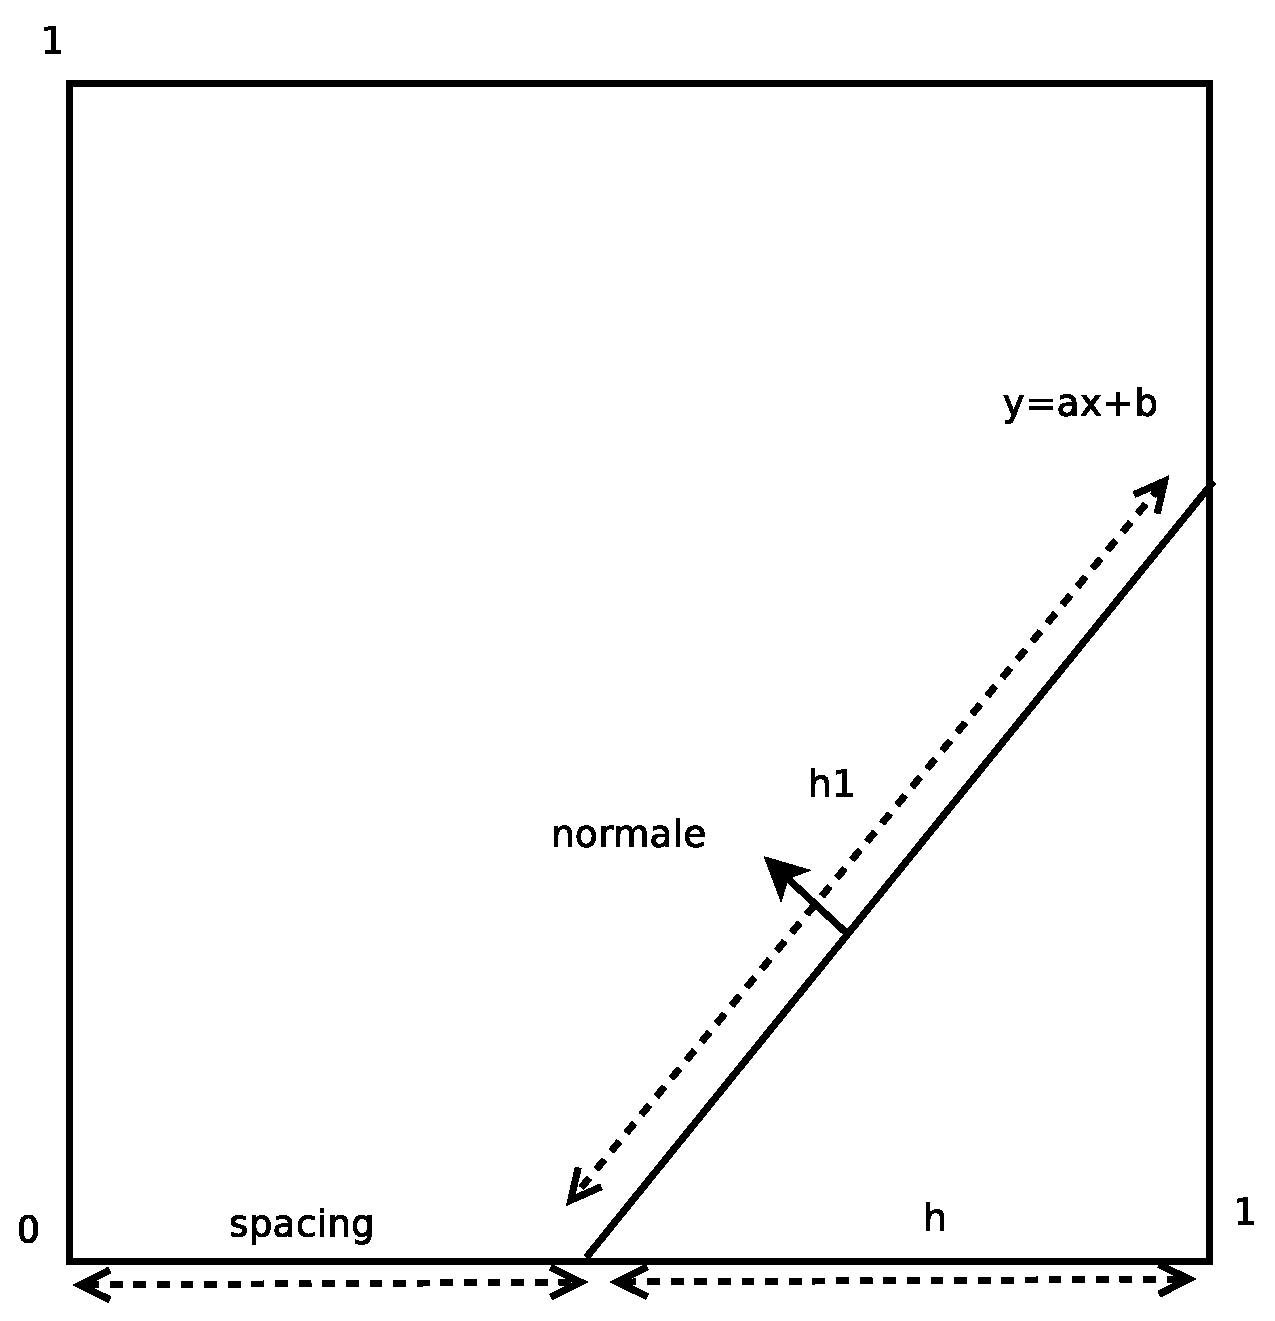
\includegraphics[width=0.65\textwidth]{img/cap2/mesh.eps}
\caption{Principali parametri di definizione per una frattura}
\end{center}
\end{figure}

\begin{Code03_01}[caption={Definizione della frattura}]
[fractureData]

spaceDimension = 1.

   [./levelSet]		// parametri di definizione del level set
     // funzione level set che rappresenta la frattura
     levelSet = y-a*x-b 			
     ylevelSet = y-a1*t-b1 			
     xlevelSet = x-a2*t-b2				          
     levelSetCut = -1	
     yMap = a1*t+b1					
     xMap = a2*t+b2				
     // fattore di scala, rapporto tra la lunghezza della mesh di integrazione e la 
     // lunghezza della mesh reale
     jacMap = [ h/h1 ]				
     normalMap = [ ]					
     integrationTypeSimplex = IM_STRUCTURED_COMPOSITE(IM_TRIANGLE(3),1)
   [../]

   [./domain]		// parametri di definizione del dominio di integrazione
     thickness = 
     spacing = x+c      	
     spatialDiscretization = n
     // dimensioni del dominio
     translateAbscissa = c
     lengthAbscissa = h1
     lengthOrdinate = 0.
     lengthQuota = 0.
     meshType = GT_PK(1,1)
     // variabili per l'integrazione
     integrationTypeVelocity = IM_GAUSS1D(3)
     integrationTypePressure = IM_GAUSS1D(2)		
     FEMTypeVelocity = FEM_PK(1,1)
     FEMTypePressure = FEM_PK(1,0)
     FEMTypeLinear = FEM_PK(1,1)
   [../]

   [./darcy]		// parametri per la definizione del problema di Darcy
     etaNormal = 0.01
     etaNormalDistribution = 1. 
     etaTangential = 100.
     etaTangentialDistribution = 1.
     source = 
     solution = 
     velocity = 
   [../]

[../]

\end{Code03_01}


\lstnewenvironment{Code03_01}[1][]{\lstset{basicstyle=\small\ttfamily, columns=fullflexible,framexrightmargin=+.1\textwidth, keywordstyle=\color{red}\bfseries, commentstyle=\color{blue},language=C++, basicstyle=\small,  numberstyle=\tiny, stepnumber=1, numbersep=5pt, frame=shadowbox, #1}}{}


\chapter{Strumenti di sviluppo}
Lo sviluppo della nostra libreria ha richiesto l'uso di strumenti specifici atti a facilitare e sistematizzare la gestione del codice quali \texttt{git}, \texttt{CMake} e \texttt{Dxygen}.\\
\href{https://github.com/}{\texttt{Git}} è un sistema di controllo versione utilizzavile direttamente da linea di comando, molto diffuso è utile per tenere traccia delle varie fasi di sviluppo del codice. Git gestisce in modo adeguato i contributi al codice provenienti da agenti esterni e permette la condivisione del codice.\\
\href{http://www.cmake.org/}{\texttt{CMake}} è un software libero multipiattaforma nato per l'automazione dello sviluppo. Sostanzialmente con l'uso di \texttt{CMake} è possibile configurare e generare Makefile per il sistema operativo in uso. Questo facilita la diffusione del codice tra sviluppatori, non dovendo far altro che lanciare \texttt{CMake} e lasciare che sia lui ad occuparsi della ricerca di compilatori e librerie locali e della costruzione di software.\\
\href{www.doxygen.org/}{\texttt{Doxygen}} è un sistema multipiattaforma molto diffuso per la generazione automatica della documentazione di un codice. Per ottenere la documentazione è necessario introdurre nel codice dei commenti con una sintassi particolare, e il risultato è contiene l’elenco delle classi implementate, i loro diagrammi di collaborazione e la descrizione di metodi ed attributi.

\section{\texttt{Git}}
Il codice del progetto è reperibile su \texttt{git} ed è possibile scaricarlo e collabolare allo sviluppo clonando il codice dalla repository  \href{https://github.com/}{\texttt{GitHub}}:\\
\begin{center}
\texttt{ git clone https://github.com/mariaiemoli/progetto.git}
\end{center}
Nella cartella principale è contenuto anche un file \texttt{.gitignore}, in cui sono specificate le estensioni dei files e le sottocartelle che non devono essere visionati in una repository \texttt{git}. In particolare non si è interessati ai files temporanei che vengono eventualmente generati dagli editor, e alle cartelle generate da uno scorretta configurazione di \texttt{Doxygen}.

\section{\texttt{CMake}}
\texttt{CMake} si basa sulla creazione di files \texttt{CMakeLists.txt} nella directory del progetto, che contengono le direttive necessarie per creare il \texttt{Makefile} per compilare ed eseguire il codice. \\
Nella directory principale si trova un primo file \texttt{CMakeLists.txt} in cui si impostano i parametri fondamentali quali la dipendenza dalla versione di \texttt{CMake}, il nome del progetto, si includono le directory dei sorgenti nel path di compilazione e si caricano le librerie esterne utilizzate dai sorgenti. \\
le librerie che vengono caricate sono:
\begin{itemize}
\item \texttt{Eigen}, libreria template per l'algebra lineare usata principalmente nella fase di imposizione delle condizioni di interfaccia sul triangolo di intersezione nel caso della biforcazione, per il modello ridotto;
\item \texttt{Getfem++}, libreria matematica per gli elementi finiti usata per scrivere e risolvere il problema numerico;
\item \texttt{Blas} (Basic Linear Algebra Subprograms) e \texttt{Qhull}, librerie necessarie per \texttt{Getfem++};
\item \texttt{Doxygen}, usato per generare la documentazione
\end{itemize}

\begin{Code03_01}
CMAKE_MINIMUM_REQUIRED( VERSION 2.8 )

PROJECT(PACS)

SET(CMAKE_CXX_FLAGS "-std=c++0x -Wall ${CMAKE_CXX_FLAGS}")

SET(CMAKE_MODULE_PATH 
	${CMAKE_SOURCE_DIR}/cmake ${CMAKE_MODULE_PATH})

# Include Eigen3
FIND_PACKAGE(PkgConfig)
PKG_CHECK_MODULES(EIGEN3 REQUIRED eigen3)
INCLUDE_DIRECTORIES(${EIGEN3_INCLUDE_DIRS})

# Include Doxygen
find_package(Doxygen)
[ ... ]

# Include Getfem
if (GETFEM_LIBRARIES AND GETFEM_INCLUDE_DIRS)
[ ... ]

#Include for BLAS library
find_package ( BLAS )
[ ... ]


#Include for LAPACK library
find_package ( LAPACK )
[ ... ]

#Include for QHULL library
set(QHULL_MAJOR_VERSION 6)
[ ... ]

SET(CMAKE_INSTALL_PREFIX 
	${CMAKE_SOURCE_DIR}/install-dir CACHE PATH "" FORCE)

ADD_SUBDIRECTORY(src)
ADD_SUBDIRECTORY(test)
\end{Code03_01}

Per poter usare \texttt{CMake} è necessario posizionarsi nella directory in cui è contenuto il progetto e creare una cartella in cui compilare il codice. Per lanciare \texttt{CMake} è necessario digitare i seguenti comandi: \\ 
%\begin{center}
 \texttt{cd $<$build\_dir$>$ } \\
\texttt{cmake $<$source\_dir$>$}
%\end{center}

\texttt{CMake} imposta le variabili di path come definito nel file  \texttt{CMakeLists.txt}, esamina le dipendenze da librerie esterne e procede esaminando le sottocartelle aggiunte nel file di configurazione. In particolare esamina le sottocartelle \texttt{src} e \texttt{test}, in cui sono presenti altri files  \texttt{CMakeLists.txt}, che impostano i rispettivi obiettivi e definiscono le rispettive sottocartelle. Questo permette a \texttt{CMake} di esaminare tutta la directory in cui è contenuto il progetto in maniera ricorsiva. \\
Nella cartella \texttt{src} il file  \texttt{CMakeLists.txt} aggiunge la creazione di una libreria a partire dal codice del progetto. 
\begin{Code03_01}
ADD_LIBRARY(pacs ${TARGET_SRC} ${TARGET_HANDLER})
\end{Code03_01}

Nella cartella test si trovano dei files data di esempio per poter eseguire il codice, contenuti della sottocartella \texttt{data}. Il file  \texttt{CMakeLists.txt} nella cartella dei test definisce gli obiettivi e i collegamenti necessari per l'esecuzione. 

\par Una volta che il \texttt{Makefile} è stato generato è possibile compilare il codice con il comando: \\ 
\texttt{make}.
Questo crea nella sottocartella \texttt{test} un eseguibile chiamato \texttt{darcy}. Per poterlo eseguire è sufficiente lanciarlo da terminale dandogli in pasto uno dei files presenti nella sottocartella \texttt{data}:\\
\texttt{ .\textbackslash darcy data\textbackslash$<$file\_data$>$ }

\section{\texttt{Doxygen}}
Per poter creare la documentazione al codice con \texttt{Doxygen} è necessario che nella cartella principale sia presente il file \texttt{Doxygen}, in caso contrario è necessario crearlo con il comando:\\
\texttt{Doxygen -g}\\
In questo file sono definite le variabili che permettono di creare la documentazione come il nome del progetto, la directory dove creare la documentazione, le cartelle dove si trovano i sorgenti e l'estensione dei files da considerare.

\begin{Code03_01}
PROJECT_NAME 				=	 Problema di Darcy in un network di fratture
OUTPUT_DIRECTORY			=	./build/doc
INPUT						= 	./src ./test
FILE_PATTERNS				= 	*.cc *.h
HAVE_DOT					=	YES
COLLABORATION_GRAPH		=	YES
HIDE_UNDOC_RELATIONS		=	NO
\end{Code03_01}

Dopo aver lanciato \texttt{CMake} è possibile generare la documentazione semplicemente eseguendo: \\
\texttt{cd $<$build\_dir$>$} \\
\texttt{make doc}

Questo crea una sottocartella \texttt{build/doc} che contiene la documentazione \texttt{html} e \LaTeX{}.
\lstnewenvironment{Code}[1][]{\lstset{basicstyle=\small\ttfamily, columns=fullflexible, framexrightmargin=+.1\textwidth, keywordstyle=\color{red}\bfseries, commentstyle=\color{blue},
language=C++, basicstyle=\small,  numberstyle=\tiny, stepnumber=1, numbersep=5pt, frame=shadowbox, #1}}{}

\chapter{Implementazione delle fratture}
Passiamo ora a descrivere le principali classi del codice che definiscono la struttura e le proprietà delle fratture, porgendo particolare attenzione alle classi modificate e a quelle da noi implementate.\\

\begin{figure}[htbp]
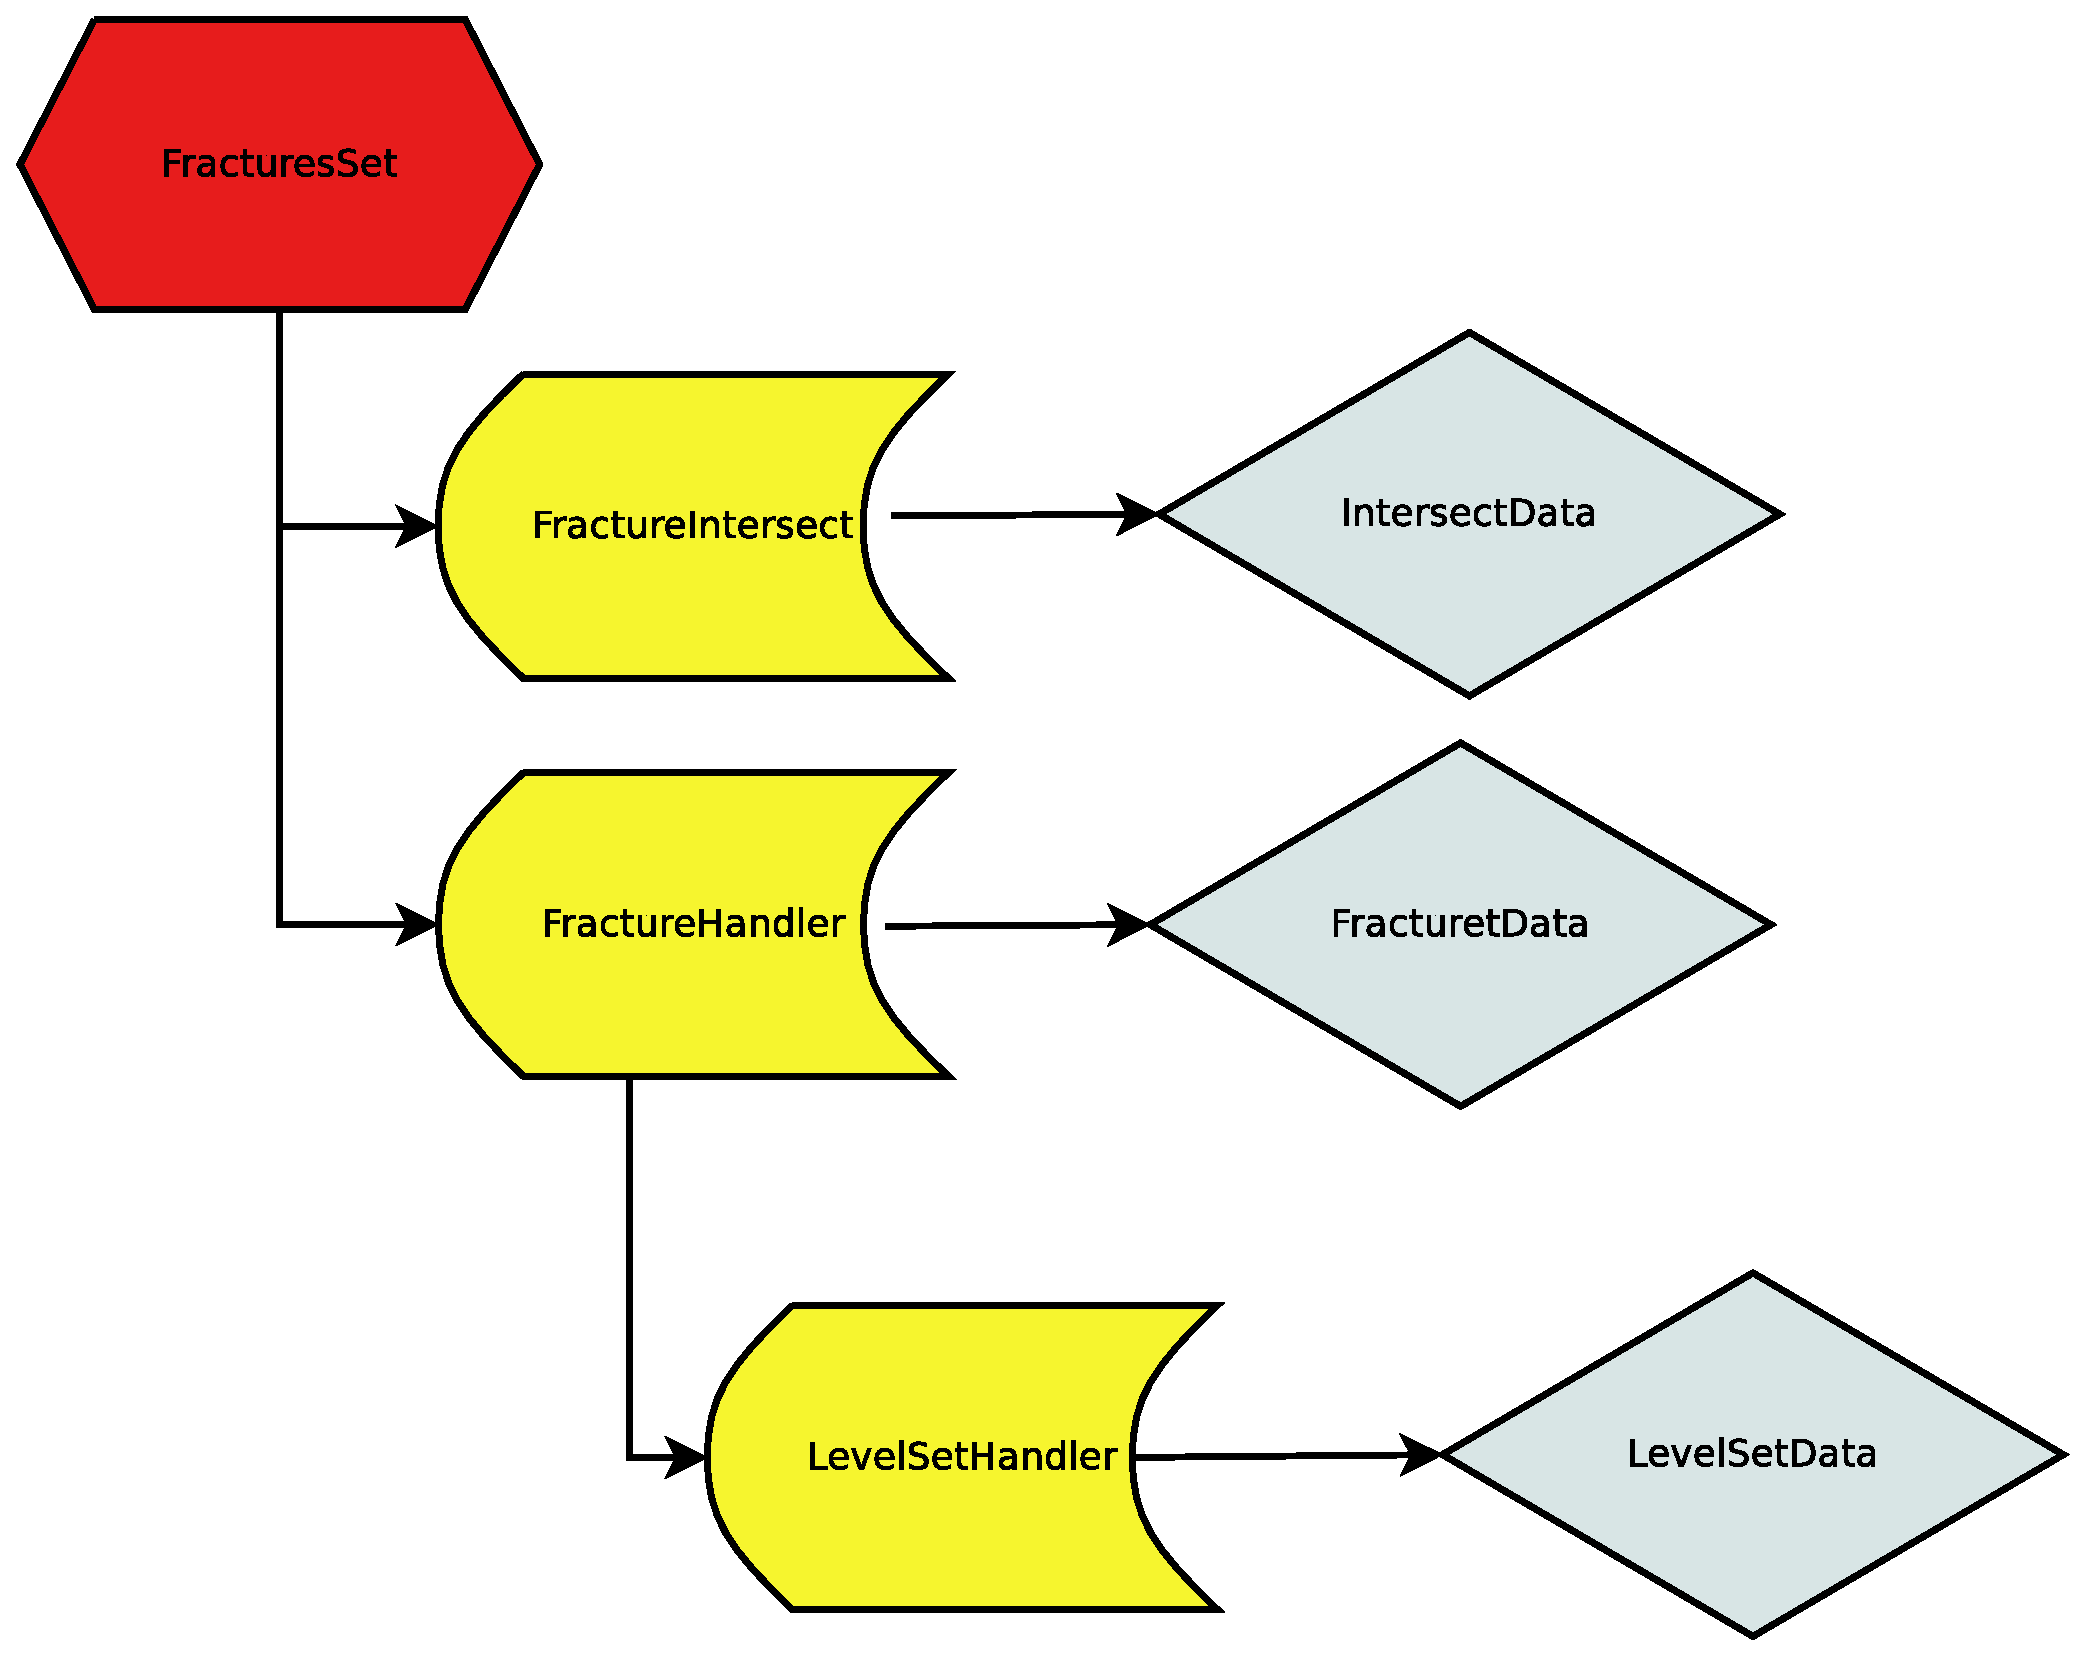
\includegraphics[width=1\textwidth]{img/fratture.eps}
\caption{Inclusione tra le varie classi che costituiscono l'insieme delle fratture}\label{Inclusione classi}
\end{figure}


\par Le classi usate per rappresentare le fratture e le intersezioni si dividono in due categorie:
\begin{enumerate}
\item[-] le classi in cui sono implementati tutti i metodi necessari per la costruzione e la manipolazione della grandezza ( insieme delle fratture, singola frattura, intersezioni, level set). Queste classi sono principalmente denominate col il suffisso \textit{Handler} e costituiscono l'ossatura dell'insieme delle fratture;
\item[-] le classi in cui sono contenuti tutti i parametri geometrici, fisici e le grandezze numeriche per l'implementazione e la risoluzione con elementi finiti, che riguardano la grandezza in esame. Vengono indicate con il suffisso \textit{Data} e rappresentano sempre un campo della corrispondente classe di tipo \textit{Handler}.
\end{enumerate}



\section{La Classe \texttt{FracturesSet}}
La class \texttt{FracturesSet} è la classe che contiente tutte le fratture e le rispettive intersezioni. La funzione che costruisce l'insieme delle fratture e le eventuali intersezioni è la funzione  \texttt{init}, che prende in input tutti i parametri necessari quali il numero di fratture, le mesh per l'integrazione e una variabile di tipo GetPot per la lettura dal file data. 

\begin{Code}[caption={Classe \texttt{FracturesSet}}]
class FracturesSet
{
public:

    enum
    {
        FRACTURE_UNCUT = 10000,
        FRACTURE_INTERSECT = 10000
    };

    FractureHandler ( const GetPot& dataFile,
                      const size_type& ID,
                      const std::string& section = "fractureData/" );

    void init ( );

    [ ... ]

private:
	FracturePtrContainer_Type M_fractures;

	FractureIntersectPtr_Type M_intersections;
	[ .... ]
};
\end{Code}
I campi principali della classe sono:
\begin{enumerate}
\item[-] \texttt{M\_fractures}, variabile di tipo vettore di puntatori alla classe \texttt{FractureHandler}  di cui parleremo più avanti, che rappresenta l'insieme di tutte le fratture;
\item[-] \texttt{M\_intersections}, un puntatore alla classe \texttt{FractureIntersect}, che rappresenta l'insieme di tutte le intersezioni. 
\end{enumerate}


\section{La Classe \texttt{FractureHandler}}

La classe  \texttt{FractureHandler} è la classe che inizializza e gestisce ogni frattura. I principali campi di questa classe sono:
\begin{enumerate}
\item[-] \texttt{M\_data}: classe \texttt{FractureData} che contiene tutte le informazioni circa la natura geometrica e fisica della singola frattura;
\item[-] \texttt{M\_levelSet}: puntatore alla classe \texttt{LevelSetHandler} di cui parleremo più avanti;
\item[-] i metodi di integrazione e le mesh per pressione e velocità;
\item[-] il vettore dei gradi di libertà estesi per velocità e pressione.
\end{enumerate}

La particolarità di questa classe è che possiede due mesh: una mesh 2d \texttt{M\_meshMapped} e una mesh 1d \texttt{M\_meshFlat}. Questo deriva dal fatto che le fratture sono su un piano e hanno una rappresentazione del tipo $y=f(x)$, cioè i loro punti hanno coordinate $(x,y)$. La libreria che noi usiamo, \textit{GetFEM++}, non è in grado di integrare su una mesh i cui punti hanno coordinate $(x,y)$ un'equazione 1d come quella del nostro modello ridotto. La tecnica è quindi quella di risolvere il problema integrando sulle mesh " piatte " 1d ottenute proiettando le mesh reali, e successivamente interpolare i risultati ottenuti per ritornare sulle mesh 2d. La creazione delle mesh è nella funzione \texttt{ init}.
\par La funzione principale di questa classe è  \texttt{setMeshLevelSetFracture }.
Tale funzione crea un legame tra la frattura corrente e le fratture con cui ha un'intersezione, tenendo traccia della mesh e dei valori del level set della frattura corrente nei punti della frattura intersecata. Nel caso di intersezione di tipo \textit{Cross}, dove l'intersezione tra due level set non è detto che avvenga su due punti delle rispettive mesh, vengono aggiunti i gradi di libertà estesi, due per la velocità e uno per la pressione. Nel caso dell'intersezione di tipo \textit{Bifurcation} l'introduzione di tali elementi non si rende necessaria.


\begin{Code}[caption={Funzione \texttt{setMeshLevelSetFracture}}]
size_type FractureHandler::setMeshLevelSetFracture ( 
					FractureHandler& otherFracture,
					size_type& globalIndex,
				         const std::string& type )
{	
[ ... ]
if ( !M_meshLevelSetIntersect[ otherFractureId ].get() )
{
   M_meshLevelSetIntersect[ otherFractureId ].reset
	 ( new GFMeshLevelSet_Type ( M_meshFlat ) );
   LevelSetHandlerPtr_Type otherLevelSet = otherFracture.getLevelSet();
   M_levelSetIntersect [ otherFractureId ].reset 
	( new GFLevelSet_Type ( M_meshFlat, 1, false )  );
   M_levelSetIntersect [ otherFractureId ]->reinit();

   const size_type nbDof = 
	M_levelSetIntersect [ otherFractureId ]->get_mesh_fem().nb_basic_dof();

   for ( size_type d = 0; d < nbDof; ++d )
   {
      base_node node = M_levelSetIntersect [ otherFractureId ]
			->get_mesh_fem().point_of_basic_dof(d);
      base_node mappedNode ( node.size() +1 );
      scalar_type t = d*1./(M_data.getSpatialDiscretization () );
      base_node P (node.size());
      P [0] = t;
      mappedNode [0] = node [0];
      mappedNode [1] = M_levelSet->getData()->y_map ( P );
      M_levelSetIntersect [ otherFractureId ]->values(0)[d] = 
	otherLevelSet->getData()->ylevelSetFunction ( mappedNode );
   }

   M_meshLevelSetIntersect[ otherFractureId ]
	->add_level_set ( *M_levelSetIntersect [ otherFractureId ] );
   M_meshLevelSetIntersect[ otherFractureId ]->adapt ();

   size_type i_cv = 0;
   dal::bit_vector bc_cv =
   M_meshLevelSetIntersect[ otherFractureId ]->linked_mesh().convex_index();
		
   for ( i_cv << bc_cv; i_cv != size_type(-1); i_cv << bc_cv )
   {
     if ( M_meshLevelSetIntersect[ otherFractureId ]->is_convex_cut ( i_cv ) )
     {  
        if ( type == "Cross")
        {	
           M_meshFlat.region ( FractureHandler::FRACTURE_UNCUT 
		* ( M_ID + 1 ) ).sup ( i_cv );
	 M_meshFlat.region ( FractureHandler::FRACTURE_INTERSECT 
		* ( M_ID + 1 ) + otherFractureId + 1 ).add( i_cv );
	 M_extendedPressure.push_back ( 
		M_meshFEMPressure.ind_basic_dof_of_element ( i_cv )[0] );
	 M_extendedVelocity.push_back ( 
		M_meshFEMVelocity.ind_basic_dof_of_element ( i_cv )[0] );
	 M_extendedVelocity.push_back ( 
		M_meshFEMVelocity.ind_basic_dof_of_element ( i_cv )[1] );
        }
            	
       M_fractureIntersectElements [ otherFractureId ].push_back ( i_cv );
	
           [ ... ]
      }
   }
}

return numIntersect;
}
\end{Code}


\section{Le Classi \texttt{LevelSetHandler} e \texttt{LevelSetData}}
Le fratture sono rappresentate come delle rette, funzioni $y=f(x)=ax+c$. Ad ogni frattura è associata una funzione level set  del tipo $f(x,y)=y-ax-b$ che divide il piano in due semipiani: i punti un cui $f(x,y)>0$ e i punti in cui $f(x,y)<0$. I punti in cui $f(x,y)=0$ sono quelli in cui è definita la frattura. 
\par La classe \texttt{LevelSetHandler} inizializza il levelset associato alla frattura. 
La funzione fondamentale della classe è la funzione \texttt{init}, funzione che inizializza il level set, definisce i metodi di integrazione e aggiunge alla mesh di supporto l'informazione legata al level set. I campi fondamentali della classe sono:
\begin{enumerate}
\item[-] \texttt{M\_data}: puntatore alla classe \texttt{LevelSetData}, classe che contiene tutte le informazioni sul level set e le funzioni per valutarne il valore nei punti;
\item[-] \texttt{M\_mesh}: puntatore ad una variabile di tipo \textit{getfem::mesh\_level\_set}, classe che contiene informazioni sulla mesh tagliata da level set;
\item[-] \texttt{M\_levelSet}: oggetto di tipo \textit{getfem::level\_set}, variabile che definisce il level set. In GetFEM un level set è rappresentato come una o due funzioni scalari, definito su una mesh di tipo \textit{getfem::mesh\_fem}, ossia una mesh su cui è definito un metodo ad elementi finiti.
\end{enumerate}

\begin{Code}[caption={Classe \texttt{LevelSetHandler}}]
class LevelSetHandler
{
public:

    LevelSetHandler ( const GetPot& dataFile, 
			const std::string& section =  "fractureData/", 
    			const std::string& sectionLevelSet = "levelSet/" );

    void init ( getfem::mesh& mediumMesh,
		    const std::string& mediumIntegrationTypeVelocity,
		    const getfem::mesh_fem& mediumMeshFEMPressure,
		    const getfem::mesh_fem& mediumMeshFEMVelocity );

	[ ... ]
private:

    LevelSetDataPtr_Type M_data;

    GFMeshLevelSetPtr_Type M_mesh;

    GFLevelSetPtr_Type M_levelSet;
	[ ... ]
};
\end{Code}


 \section{Le Classi \texttt{FractureIntersect} e \texttt{IntersectData}}

La classe \texttt{FractureIntersect} rappresenta tutte le intersezioni tra le fratture. Ad ogni tipo di intersezione viene associato il vettore delle classi \texttt{IntersectData}, classe che rappresenta la vera e propria intersezione, tenendo traccia delle informazioni sulle fratture e dell'id dell'elemento della mesh di supporto in cui avviene l'incontro.
\par Le intersezioni vengono classificate come \textit{Parallel}, \textit{Cross} e \textit{Bifurcation}.  L'idea alla base della classificazione è quella di considerare gli elementi della mesh 2d di supporto, la mesh del mezzo, in cui passano due o più fratture, e di associargli un flag:
\begin{enumerate}
\item[-] \textit{Parallel}: quando due o più fratture passano in uno stesso elemento della mesh ma non si intersecano;
\item[-] \textit{Cross}: quando due fratture passano nello stesso elemento della mesh e si intersecano formando una \textit{X};
\item[-] \textit{Bifurcation}: quando tre fratture si intersecano in un punto comune formando una \textit{Y}.
\end{enumerate}

\begin{Code}[caption={Funzione \texttt{constructIntesection}}]
void FractureIntersect::constructIntesection ( 
	const getfem::mesh& mesh, getfem::mesh_level_set& meshLevelSet, 
	const FracturePtrContainer_Type& fractures )
{
[ ... ]
meshLevelSet.find_level_set_potential_intersections ( 
			listOfConvex, listOfLevelSet_bitVector );

sizeVectorContainer_Type listOfLevelSet ( listOfConvex.size() );

if( listOfConvex.size() > 0 )
{
   for ( size_type i = 0 ; i < listOfConvex.size(); ++i )
   {
      // Conversione da un vettore di bit a un vettore di interi
      fromBitVectorToStdVector ( 
      listOfLevelSet_bitVector [ i ], listOfLevelSet [ i ] );

       // Per ogni elemento della mesh di supporto in cui passano 
      // almeno due fratture verifico il tipo di intersezione
       IntersectionType type = intersectionType ( 
		meshLevelSet, listOfConvex [ i ], listOfLevelSet [ i ] );
	        
       // Prendo i puntatori alle fratture coinvolte
      FracturePtrContainer_Type fracturesInvolved ( listOfLevelSet[i].size() );

      for ( size_type f = 0; f < fracturesInvolved.size(); ++f )
      {
	 fracturesInvolved [ f ] = fractures [ listOfLevelSet [ i ] [ f ] ];
       }
       // Costruisco la classe IntersectData per la nuova intersezione 
       // e la aggiungo in base al tipo
      IntersectData intersection;
      intersection.setIntersection ( listOfConvex[i], fracturesInvolved );		
      M_intersections [ type ].push_back ( intersection );
    }
[ ... ]
}

\end{Code}

\par La funzione  \texttt{constructIntesection} contiene la classificazione delle intersezioni. In questa funzione viene data una numerazione globale alle intersezioni, prima quelle di tipo \textit{Cross} e poi quelle di tipo  \textit{Bifurcation}.  Nel caso delle prime vengono aggiunte due nuove incognite, una per ogni frattura, necessarie per imporre le condizioni d'interfaccia nella formulazione debole del problema. Queste nuove variabili rappresentano la pressione nel punto di intersezione e  vengono poi accoppiate in modo da risultare uguali. Nel secondo caso invece si introduce una sola incognita per ogni intersezione, variabile che rappresenta la pressione nel punto d'incontro. Per ogni frattura coinvolta inoltre si tiene traccia del grado di libertà in cui avviene l'intersezione. Questo perchè, come vedremo, la condizione al contorno deve essere imposta solo del grado di libertà dell'estremo libero della frattura.

\section{Le Classi \texttt{BC} e \texttt{BCHandler}}
%\subsection{Definizione della classe e costruttore}
La classe \texttt{BC} ci permette di imporre le condizioni al bordo in ogni singola frattura. Per ogni frattura è necessario imporre due condizioni al contorno\\ 

%\newpage	
\begin{Code}[caption={Classe \texttt{BC}}]
class BC
{
 public:

    enum
    {
        DIRICHLET_BOUNDARY_NUM = 40,
        NEUMANN_BOUNDARY_NUM = 50
    };

    // Costruttore
    BC ( getfem::mesh& mesh,
         const std::string& MeshType,
         const sizeVector_Type DOFs,
         const ElementDimension& dimension = MEDIUM );

 private:

    getfem::mesh_fem M_meshFEM;
    
    sizeVector_Type M_dirichlet;
    sizeVector_Type M_neumann;
    sizeVector_Type M_extBoundary;   
};
\end{Code}

Quando si considera una frattura priva di intersezioni o con solo intersezioni di tipo \textit{Cross} le condizioni al contorno vengono imposte rispettivamente sul primo e l'ultimo gradi di libertà della mesh.\\
Nel caso della biforcazione, invece, bisogna accertarsi di imporre le condizioni al bordo solamente nell' estremo libero, ovvero quello in cui non sia presente alcuna intersezione. 
Per far questo motivo quando costruiamo l'insieme delle intersezioni per ogni frattura salviamo un vettore contenente l'indice dei gradi di libertà in cui c'è un'intersezione.

La classe \texttt{BCHandler} viene usata per gestire le condizioni al contorno sulle fratture.

\lstnewenvironment{Code03_03}[1][]{\lstset{basicstyle=\small\ttfamily, columns=fullflexible,framexrightmargin=+.1\textwidth, keywordstyle=\color{red}\bfseries, commentstyle=\color{blue},language=C++, basicstyle=\small, numbers=left, numberstyle=\tiny, stepnumber=1, numbersep=5pt, frame=shadowbox, #1}}{}

\chapter{Classi per la gestione dell'intersezione}

Nel modello che abbiamo preso in considerazione noi le fratture hanno una rappresentazione in $\mathbb{R}$ e, nel caso della \textit{Biforcazione}, hanno un unico punto in comune. 
Nella rappresentazione 2D, invece, la regione in comune è un triangolo. \\

\begin{figure}[htbp]
\centering
\includegraphics[scale=.5]{img/subcap3_3/TriangoloBiforcazione.eps}
%\includegraphics[width=0.65\textwidth]{img/TriangoloBiforcazione.eps}
\caption{Struttura della biforcazione 2D}\label{Biforcazione}
\end{figure}

Il nostro modello trascura ovviamente delle informazioni, ma nel caso di fratture con uno spessore sufficientemente piccolo rispetto a quelle del dominio, può essere considerato una buona approssimazione della realtà.\\

Per ricavare le condizioni d'interfaccia nel caso della biforcazione per modello ridotto passiamo per la rappresentazione in $\mathbb{R}^{2}$.
Nel caso 2D le fratture hanno uno spessore e possiamo delimitare un triangolo di intersezione unendo i punti di incontro dei loro bordi. \\
Presi \textbf{N} il vettore delle normali ai lati del triangolo, \textbf{$K_{I}$} la matrice di permeabilit\`{a} all'intersezione e una costante \textit{t} possiamo definire:
\begin{center}
	$ S = \textit{t} \, diag( \textbf{N}$ \textbf{$K_{I}$} $ \textbf{N}^{T} ) $
\end{center}
Definite ora \textbf{C} matrice dei vettori che uniscono il baricentro, punto C, del triangolo con il punto medio  di ogni lato e \textbf{$P_{c}$} matrice di proiezione sullo spazio nullo della matrice di base per \textbf{C}, possiamo trovare la matrice di trasmissibilit\`{a}:
\begin{center}
	$ T = \frac{1}{\textbf{I}}( \textbf{N}$ \textbf{$K_{I}$} $ \textbf{N}^{T} ) + $\textbf{$P_{c}$} $\textbf{S}$\textbf{$P_{c}$}
\end{center}
%\textbf{u} = \left\lbrace \u_{0}, \u_{1}, \u_{2} \right\rbrace
%$\textbf{\pi} = \left\lbrace \pi_{0}, \pi_{1}, \pi_{2} \right\rbrace $
Le variabili con cui ci troviamo a lavorare sono:
	\begin{enumerate}
	\item[-] \textbf{u} : vettore dei flussi
	\item[-] $p_{I}$ :  pressione nel punto di intersezione delle assi delle tre fratture;
	\item[-] \textbf{$\pi$}: vettore delle pressioni nel punto di incontro fra l'asse della frattura i-esima con un lato del triangolo;
	\end{enumerate} 
e le condizioni che dobbiamo porre all'intersezione sono:
\begin{center}			
	$\left \{
		\begin{array}{l}	
	 		\textbf{u} - p_{I}T\textbf{1}_{3}+T \boldsymbol{\Pi}=0  \\ \\
     	 	\displaystyle \sum_{k=0}^2 u_{k} = p_{I} - \pi  \\
		\end{array}
	\right.$
\end{center} \label{condizioni d'interfaccia}

\noindent  Queste sono le condizioni d'interfaccia che verranno imposte nel punto di intersezione delle fratture.\\ 
\par In questa parte di codice per gestire sia il calcolo delle matrici introdotte precedentemente, che i punti e la geometria del triangolo di intersezione, abbiamo usato la libreria matematica \textit{Eigen}.\\
\par Note le basi teoriche possiamo passare a descrivere le principali classi del codice che definiscono la struttura e le propriet\`{a} della biforcazione in uno spazio bidimensionale.

\newpage
\begin{figure}[htbp]
\centering
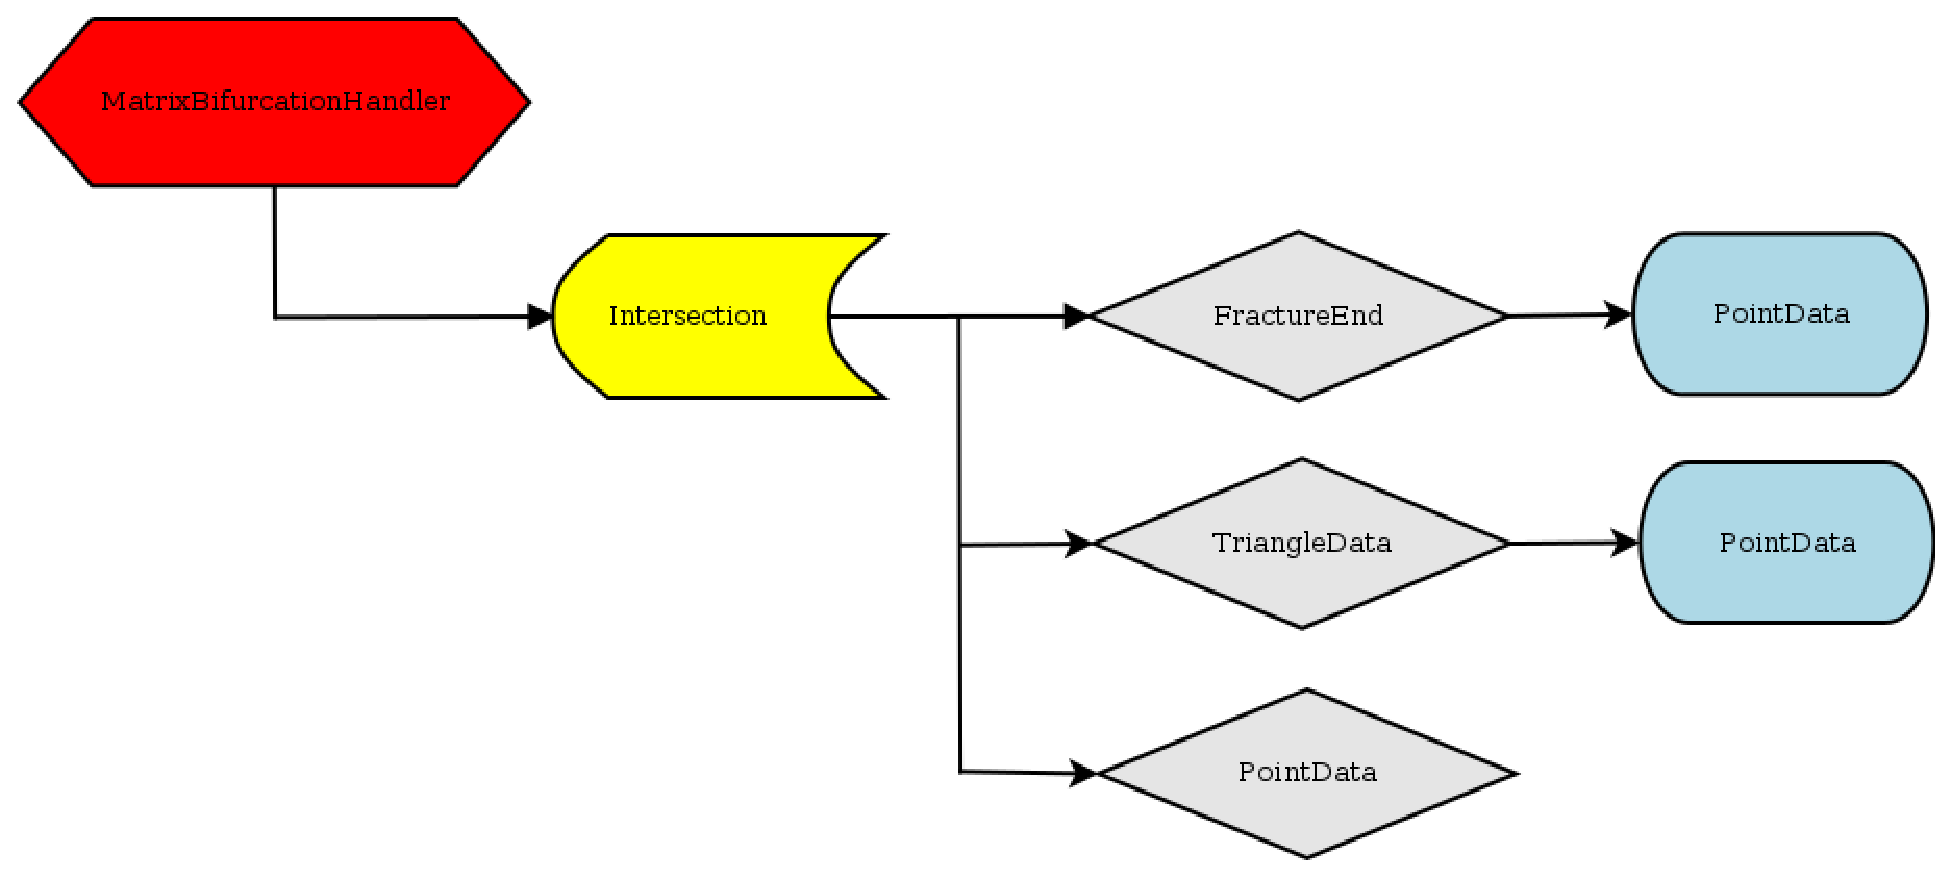
\includegraphics[height=7cm, width=1\textwidth]{img/subcap3_3/MatrixBifurcationHandler2.eps}
\caption{Inclusione tra le varie classi che costituiscono il triangolo di intersezione}\label{Inclusione classi MatrixBifurcationHandler}
\end{figure}

\section{La Classe \texttt{MatrixBifurcationHandler}}
La classe \texttt{MatrixBifurcationHandler} contiene le matrici associate a una biforcazione e implementa i metodi per calcolarle.  Il fine ultimo è il calcolo della matrice di trasmissibilità T.

\noindent I campi fondamentali della classe sono:
	\begin{enumerate}
	\item[-] \texttt{M\_intersection}: di tipo Intersection, contiene tutte le informazioni base per poter ricavare le matrici;
	\item[-] \texttt{M\_T}: matrice T di trasmissibilità necessaria per l'imposizione delle condizioni di interfaccia.
	\end{enumerate} 
\begin{Code03_03}[caption={Classe \texttt{Intersection}}]
class MatrixBifurcationHandler
{
 public:
	MatrixBifurcationHandler( const GetPot& dataFile,
				const std::string& section = "mediumData/",
				const std::string& subsection = "darcy/");
	
	void setMatrices ( FracturePtrContainer_Type& fractures );
	
	[ ... ]
	
	void computeT( scalar_type t=6.0 );

	[ ... ]

 private:

	Matrix2d M_K;
	Intersection_Type M_intersection;
	Matrix32 M_N;
	Matrix32 M_C;
	Matrix32 M_Qc;
	Matrix3d M_Pc;
	Matrix3d M_T;
};
\end{Code03_03}

\section{La Classe \texttt{Intersection}}

La class \texttt{Intersection}, definita in \texttt{Geometry.h}, contiene tutte le informazioni relative ad una biforcazione in uno spazio 2D necessarie per il calcolo delle matrici associate al triangolo di intersezione.
I campi fondamentali della classe sono:
	\begin{enumerate}
	\item[-] \texttt{M\_intersection}: di tipo PointData, rappresenta il punto di intersezione;
	\item[-] \texttt{M\_tangents}: vettore contenente le tangenti alle fratture coinvolte;
	\item[-] \texttt{M\_normals}: vettore contenente le normali alle fratture coinvolte;
	\item[-] \texttt{M\_intersectionTriangle}:di tipo TriangleData, rappresenta il triangolo di intersezione, i cui vertici sono i punti d'incontro dei bordi delle fratture.
	\end{enumerate} 

\begin{Code03_03}[caption={Classe \texttt{Intersection}}]
class Intersection
{
 public:
	[ ... ]
	
	void setIntersection( FracturePtrContainer_Type& M_FracturesSet );
	
	[ ... ]
 private:
	
	[ ... ]	
	
	PointData M_intersection;
	
	Vector2d M_tangents [ 3 ];
	Vector2d M_normals [ 3 ];
	
	TriangleData M_intersectionTriangle;
};	
\end{Code03_03}

\section{Classe \texttt{PointData} e Classe \texttt{TriangleData}}
Queste classi rappresentano un punto e un triangolo come grandezze geometriche.
Il punto geometricamente viene rappresentato come una grandezza zero dimensionale con due variabili, una \textit{x} e una \textit{y}.
Un triangolo è invece  rappresentato geometricamente dai punti che lo costituiscono.\\
\noindent La classe \texttt{PointData} ci permette di definire un punto e di poterlo manipolare con le operazioni di somma, differenza e prodotto.\\
\noindent La classe \texttt{TriangleData} ci permette di definire un triangolo e di calcolarne l'area. Inoltre sono stati implementati i metodi necessari per la costruzione del triangolo di intersezione.

\lstnewenvironment{Code03_04}[1][]{\lstset{basicstyle=\small\ttfamily, columns=fullflexible,framexrightmargin=+.1\textwidth, keywordstyle=\color{red}\bfseries, commentstyle=\color{blue},language=C++, basicstyle=\small, numbers=left, numberstyle=\tiny, stepnumber=1, numbersep=5pt, frame=shadowbox, #1}}{}

\chapter{Soluzione del problema numerico}

Passiamo ora a descrivere le principali classi del codice per la soluzione del problema numerico.

\begin{figure}[h!]
\centering
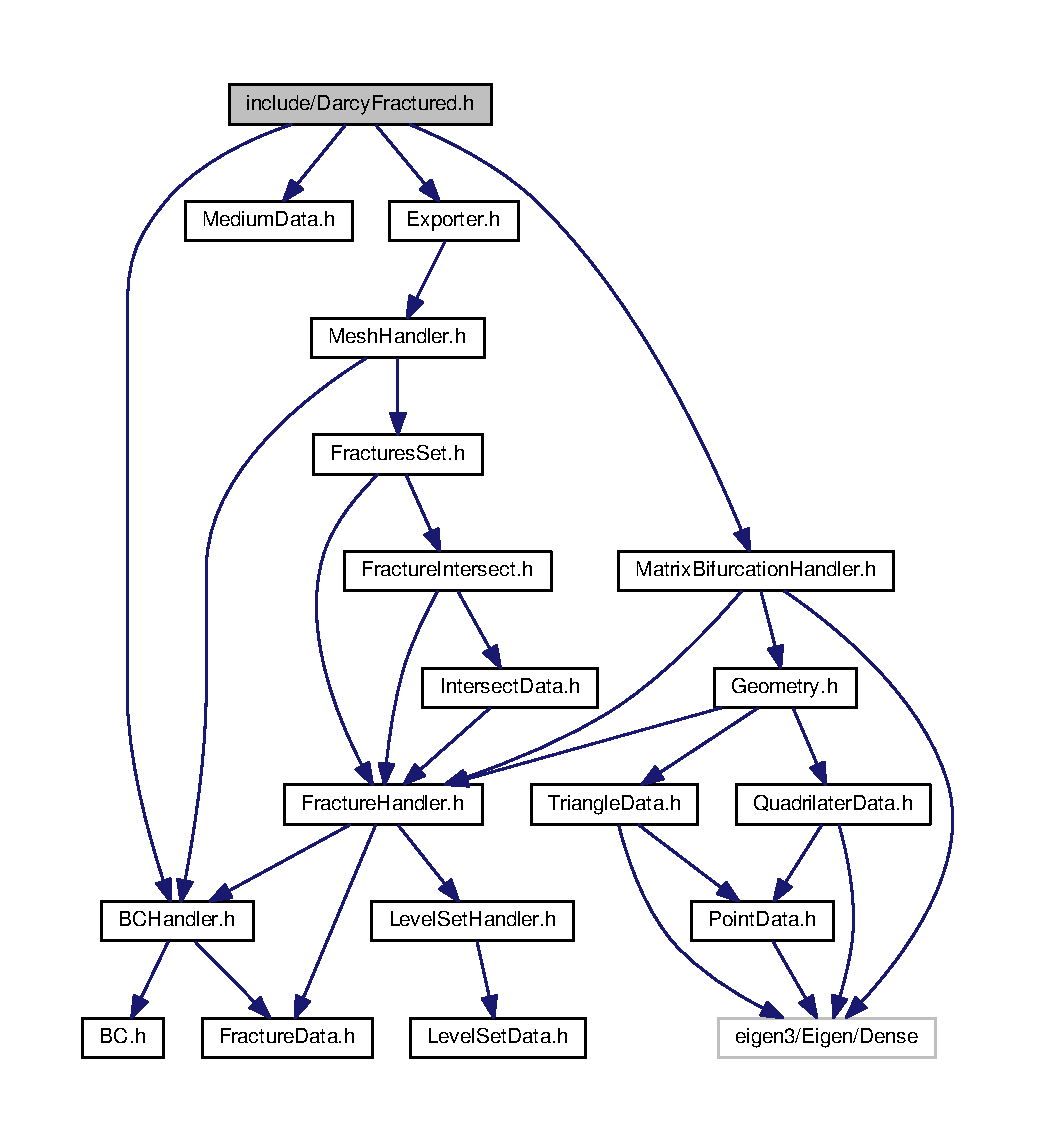
\includegraphics[scale=.59]{img/subcap3_4/DarcyFractured.pdf}
\caption{Inclusione tra le varie classi per la soluzione del problema numerico}\label{Inclusione classi DarcyFractured}
\end{figure}

\section{La Classe \texttt{DarcyFracture}}
La classe \texttt{DarcyFracture} permette di definire il problema di Darcy su ogni frattura, imporre le condizioni per le eventuali intersezioni, assemblare il sistema algebrico globale $ Ax=b $ del problema e risolverlo.\\

%Il suo costruttore richiede i seguenti parametri:
%	\begin{itemize}
%	\item \textit{Mesh:} relativa al mezzo o a una delle fratture
%	\item \textit{Stringa:} contenente il tipo di mesh di GetFem del elemento precedente
%	\item \textit{Vettore:} nullo, se la mesh fa riferimento al mezzo, contenete gli indici dei gradi di libert\`{a} degli estremi, se si sta lavorando su una frattura
%	\item \textit{ElementDimesion:} dimensione in cui stiamo lavorando ( di defaul 2 per il mezzo e 1 per le fratture)
%	\end{itemize}
\noindent I campi fondamentali della classe sono:
	\begin{enumerate}
	\item[-] \texttt{M\_globalMatrix}, matrice sparsa che rappresenta la matrice globale del sistema;
	\item[-] \texttt{M\_globalRightHandSide}, vettore del termine noto;
	\item[-] \texttt{M\_velocityAndPressure}, vettore soluzione delle velocit\'{a} e della pressione.
	\end{enumerate} 

\begin{Code03_04}[caption={Classe \texttt{DarcyFracture}}]
class DarcyFractured
{
 public:
    DarcyFractured ( const MediumDataPtr_Type& medium,
                     const MeshHandlerPtr_Type& mesh,
                     const BCHandlerPtr_Type& bcHandler,
                     const FracturesSetPtr_Type& fractures,
                     const ExporterPtr_Type& exporter );
    
    void init ( );
    
    void assembly ( const GetPot& dataFile );

    void solve ( );

	[ ... ]

 private:

	[ ... ]

    sparseMatrixPtr_Type M_globalMatrix;

    scalarVectorPtr_Type M_globalRightHandSide;

    scalarVectorPtr_Type M_velocityAndPressure;

    [ ... ]
};
\end{Code03_04}

\begin{figure}[h!]
\centering
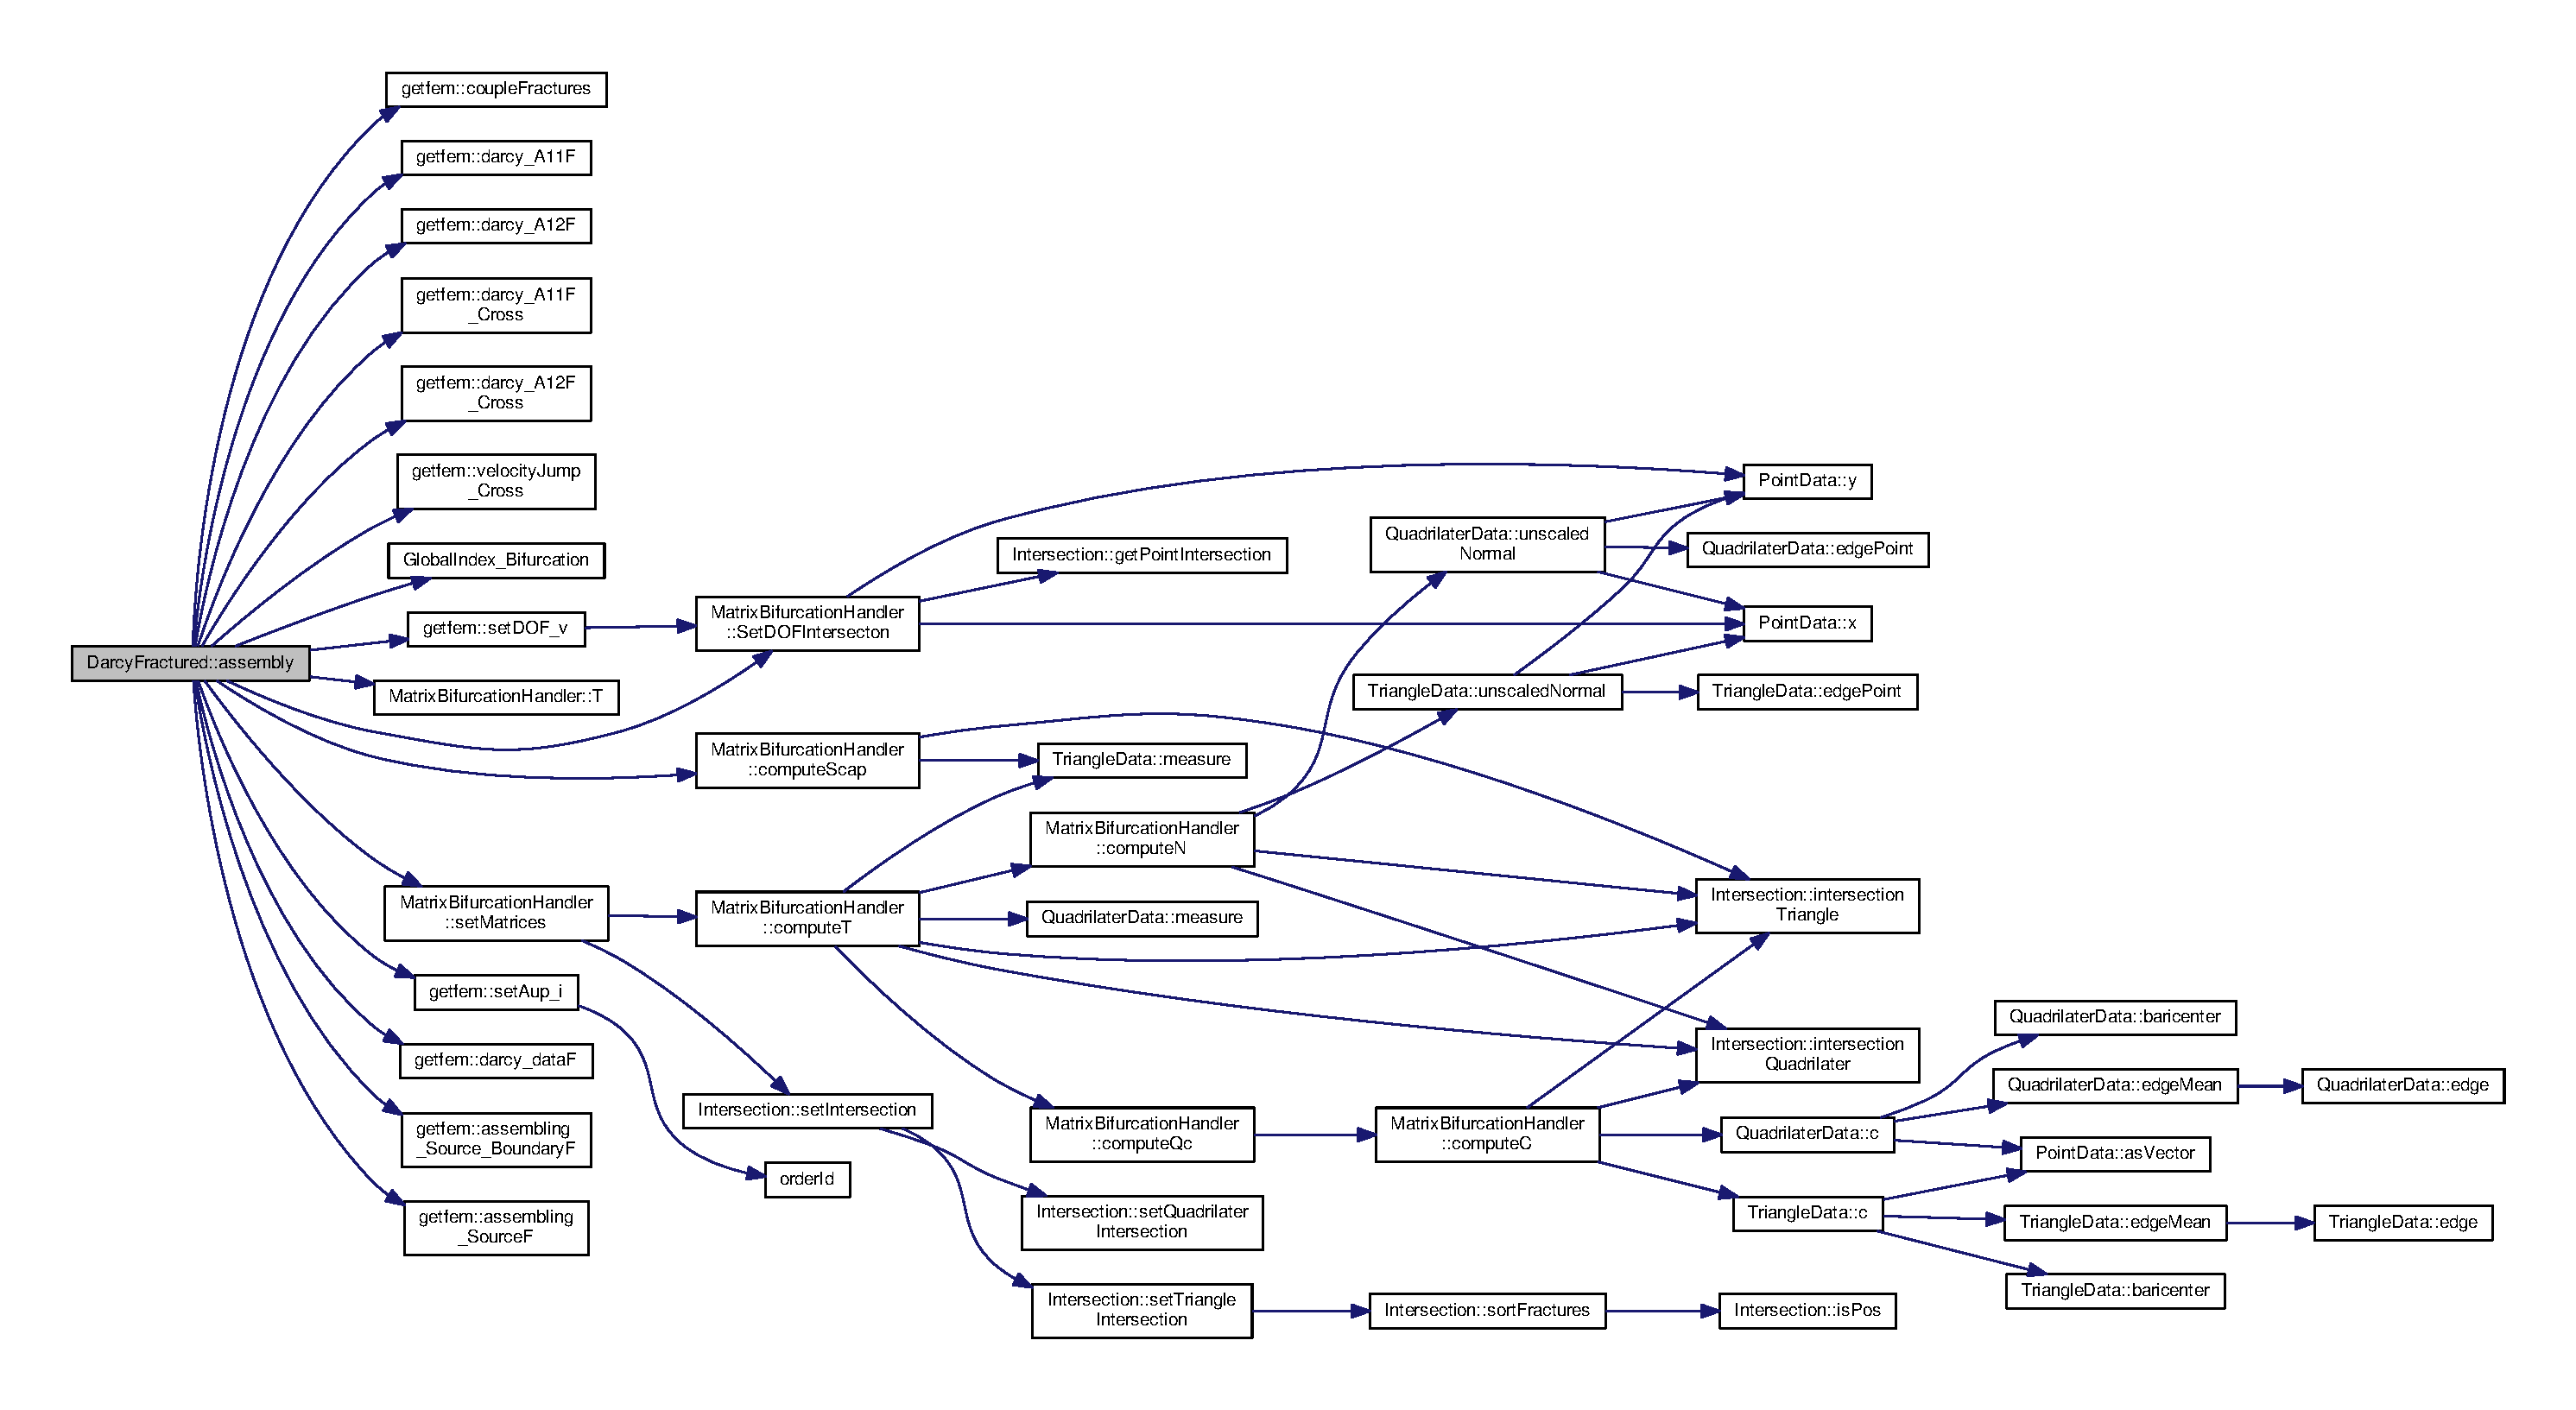
\includegraphics[scale=.4, angle=90]{img/subcap3_4/assembly.pdf}
\caption{Struttura del codice per la funzione \texttt{assembly}}\label{Inclusione classi DarcyFractured}
\end{figure}


Le funzioni fondamentali della classe sono il metodo \texttt{assembly ()} e il metodo \texttt{solve ()}. \\
\noindent Il metodo \texttt{assembly ()} crea la matrice globale $A$ e il termine noto di destra, utilizzando le funzioni della classe \texttt{XFEMOperators}. 
La matrice globale del sistema ha una struttura a blocchi, dove ad ogni frattura corrisponde un blocco derivante dal sistema \ref{sistemaAlgebrico}. Una volta definite le forme bilineari e i blocchi della matrice corrispondenti alle singole fratture, vanno imposte le condizioni d'interfaccia nel caso di eventuali intersezioni.\\
\noindent Nel caso di un \textit{Cross} si impongono le condizioni di interfaccia in maniera debole tramite le matrici $E_{2}$ e $E_{3}$, che impongono il salto di velocità nell'intersezione.\\
\noindent Nel caso di una \textit{Bifurcation} si impongono in maniera forte le condizioni di interfaccia \ref{condizioni d'interfaccia}.\\
Ipotizzando di essere in una situazione dove tre fratture hanno un intersezione di tipo \textit{Bifurcation} e una di queste si incontra con una quarta creando un intersezione di tipo \textit{Cross}, la matrice globale avrà il seguente volto:\\
%---->DA SISTEMAREEEEE <----------------- 
 \begin{center}
  $ \left[ \begin{matrix}
 			A_{0} &  B_{0} & 0 & 0 & 0 & 0 & 0 & 0 & 0 & 0\\ 
 			B_{0}^{T} & 0 & 0 & 0 & 0 & 0 & 0 & 0 & 0 & 0\\
 			0 & 0 & A_{1} &  B_{1} & 0 & 0 & 0 & 0 & 0 & 0 \\ 
		 	0 & 0 & B_{1}^{T} & 0 & 0 & 0 & 0 & 0 & 0 & 0 \\
		 	0 & 0 & 0 & 0 & A_{2} &  B_{2} & 0 & 0 & E_{2} & 0\\ 
		 	0 & 0 & 0 & 0 & B_{2}^{T} & 0 & 0 & 0 & 0 & 0\\
		 	0 & 0 & 0 & 0 & 0 & 0 & A_{3} &  B_{3} & 0 & E_{3} \\ 
 			0 & 0 & 0 & 0 & 0 & 0 & B_{3}^{T} & 0 & 0 & 0\\
 			0 & 0 & 0 & 0 & 0 & 0 & 0 & 0 & App_{0} & App_{1} \\
 			0 & 0 & 0 & 0 & E_{2}^{T} & 0 & E_{3}^{T} & 0 & 0 & 0\\
 			\end{matrix}.\right] $ 
  \end{center}
Infine il metodo \texttt{solve ()} risolve il problema e esporta i risultati ottenuti in formato \emph{vtk} per entrambe le incognite.\\

%\section{Class \texttt{XFEMOperetors}}
%Ogni frattura ha associata la matrice:
%\begin{center} 
% $ \left[ \begin{matrix}
% 	A11 &  A12 \\ 
% 	A12^{T} & 0
% \end{matrix}\right] $
%\end{center} 
%
%La classe \texttt{XFEMOperators} implementa le funzioni che ci permettono di calcolare questi blocchi.
%Le sue funzioni principali sono le seguenti:
%
%\begin{Code03_03}[caption={Funzioni per assemblare la matrice globale}]
%//Costruisce  A11 = Aij = a(\phi_j, \phi_i)
%void darcy_A11F ( sparseMatrixPtr_Type& M,
%                  const FractureHandlerPtr_Type& fracture,
%                  const scalar_type& gammaU,
%                  const scalarVector_Type& invKTangentialInterpolated,
%                  const sizeVector_Type &ExtBoundary,
%                  const size_type& uncutRegionFlag );
%
%// Aggiorna A11 nel caso intersezione" Cross "
%void darcy_A11F_Cross ( sparseMatrixPtr_Type& M,
%					    const FractureHandlerPtr_Type& fracture,
%					    const scalarVector_Type& invKTangentialInterpolated,
%					    const FractureHandlerPtr_Type& otherFracture,
%					    const size_type& cutRegionFlag );
%
%//Costruisce A12 = Bij = b(\phi_j, \omega_i)
%void darcy_A12F ( sparseMatrixPtr_Type& M,
%                  const FractureHandlerPtr_Type& fracture,
%                  const size_type& uncutRegionFlag );
%
%//Aggiorna A12 = Bij = b(\phi_j, \omega_i) nel caso di intersezione " Cross "
%void darcy_A12F_Cross ( sparseMatrixPtr_Type& M,
%                  	    const FractureHandlerPtr_Type& fracture,
%                  	    const FractureHandlerPtr_Type& otherFracture,
%                  	    const size_type& cutRegionFlag );
%\end{Code03_03}
%
%Altre importanti funzioni sono quelle che ci permetto di costruire il termine noto e son sempre contenute in questa classe.

\chapter{Costruzione del file Data} 
\section{Caso particolare: biforcazione con due fratture}

Come ultimo caso di studio ci siamo concentrate sulla biforcazione generata da due fratture. 

\begin{figure}[htbp]
\begin{center}
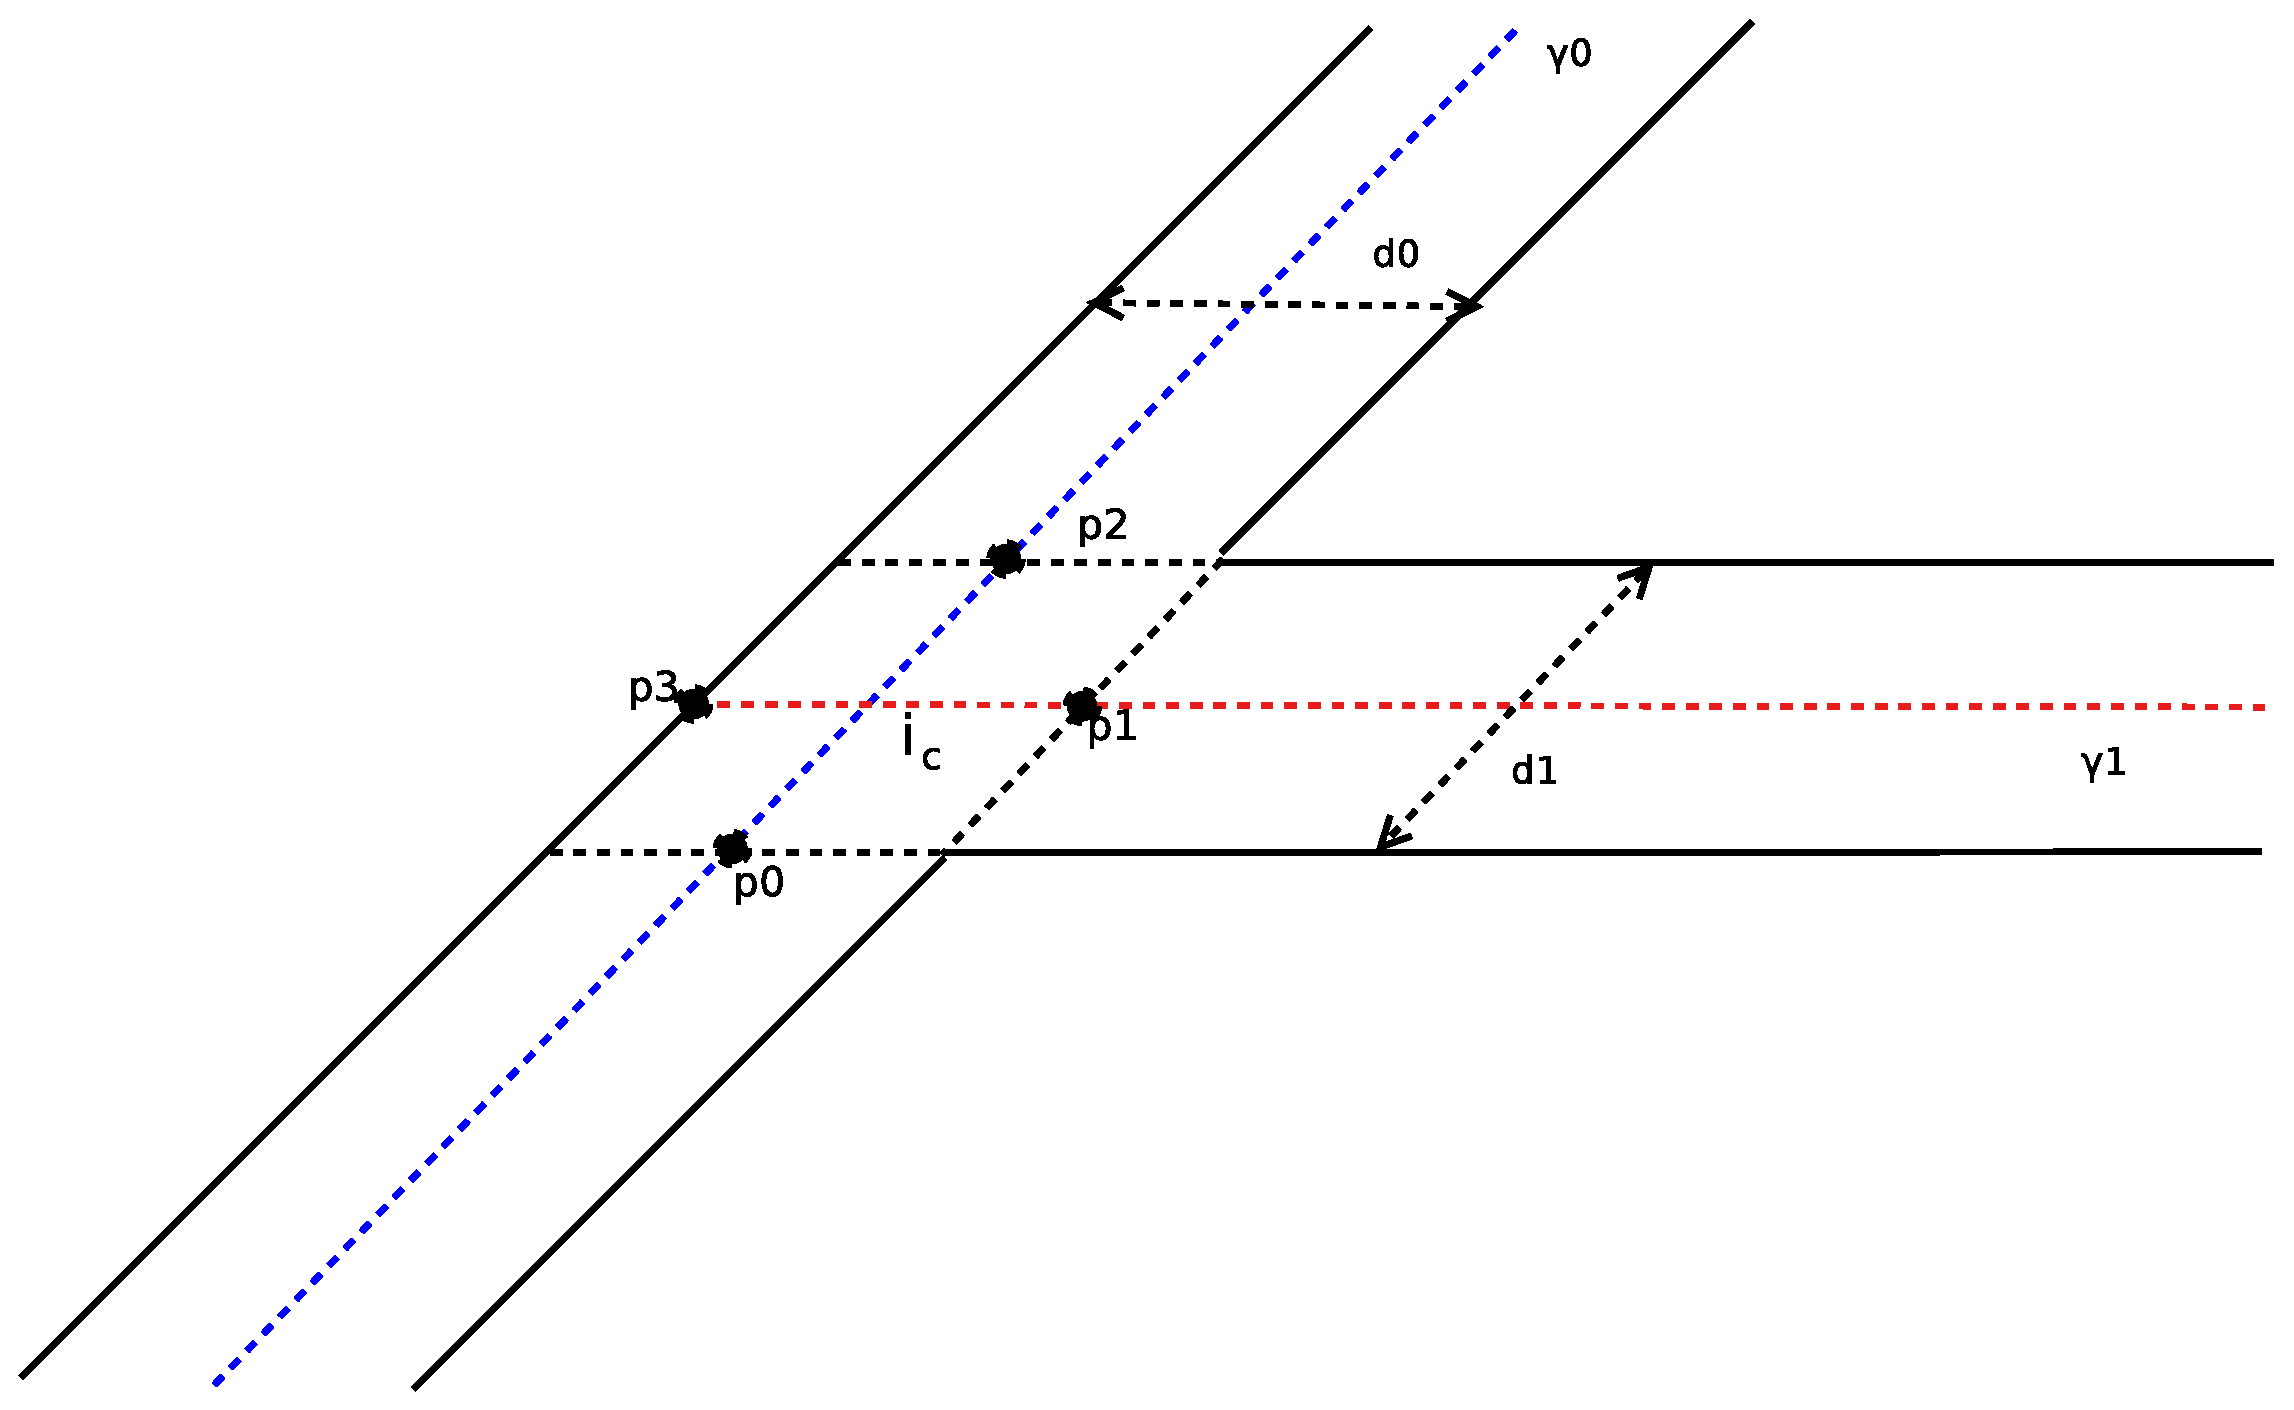
\includegraphics[width=0.8\textwidth]{img/cap6/y.eps}
\caption{Struttura di un'intersezione di tipo \textit{Bifurcation} tra due fratture.}\label{Y}
\end{center}
\end{figure}

A differenza di quando visto fino ad ora, qui la regione d'intersezione non è più un triangolo, ma un parallelogramma. Si può generalizzare l'approssimazione fatta con gli operatori mimetici, essendo degli operatori generici, non legati al tipo di cella di integrazione su cui si lavora. \\
\noindent Il punto di intersezione $i_c$ rappresenta un punto generico per la frattura $\gamma_0$ in figura \ref{Y}, mentre per la frattura $\gamma_1$ rappresenta il primo o l'ultimo nodo. Questo punto non è detto che coincida con un nodo della mesh $\gamma_0$ , in generale non sappiamo dove cadrà, per questo per poter imporre le condizioni d'interfaccia in modo corretto abbiamo introdotto per quesa frattura due gradi di libertà estesi per la velocità e uno per la pressione. In questo modo possiamo ottenere una miglior approssimazione del valore di velocità e pressione prima e dopo il punto di intersezione nell'elemento della mesh tagliato. \\
Esteso il codice di partenza per la costruzione del quadrilatero di intersezione, le condizioni d'interfaccia che vanno imposte hanno la stessa forma del caso delle tre fratture:

\begin{center}			
	$\left \{
		\begin{array}{l}	
	 		\textbf{u} - p_{I}T\textbf{1}_{3}+T \boldsymbol{\Pi}=0  \\ \\
     	 	\displaystyle \sum_{k=0}^2 u_{k} = p_{I} - \pi  \\
		\end{array}
	\right.$
\end{center} \label{condizioni d'interfaccia y }

\noindent In questo caso cambiano però le dimensioni. La matrice di trasmissibilità $T$ è ora una matrice di $\mathbb{R}^{4 \times 4}$, come diretta conseguenza della natura delle matrici $C$ e $N$. Ora infatti l'area d'intersezione è delimitata da quattro lati. Anche lo scalare $\pi$ e il vettore $\boldsymbol{\Pi}$ cambiano, e diventano:
$$\boldsymbol{\Pi} = \left[ \begin{matrix}
 			p_0\\ 
 			p_1\\
 			p_2 \\ 
		 	p_3 \\
 			\end{matrix}\right] 
$$ 
 e
$$ \pi = \frac{p_0 + p_1 + p_2 + p_3 }{4} $$

Per poter imporre le condizioni d'interfaccia, per la frattura tagliata, è necessario usare il valore della pressione e della velocità a ridosso dell'intersezione, ma questi valori sono incogniti. 
Usiamo il grado classico di pressione e il grado esteso per indicare il valore di pressione prima e dopo il punto $i_c$, indicati con $p_0$ e $p_2$ in figura \ref{Y}.  L'incognita $p_1$ rappresenta il primo o l'ultimo grado di libertà della frattura $\gamma_1$, mentre con $p_3$ indichiamo un nodo fittizio, in cui imponiamo condizione di flusso nullo. 

\begin{figure}[htbp]
\begin{center}
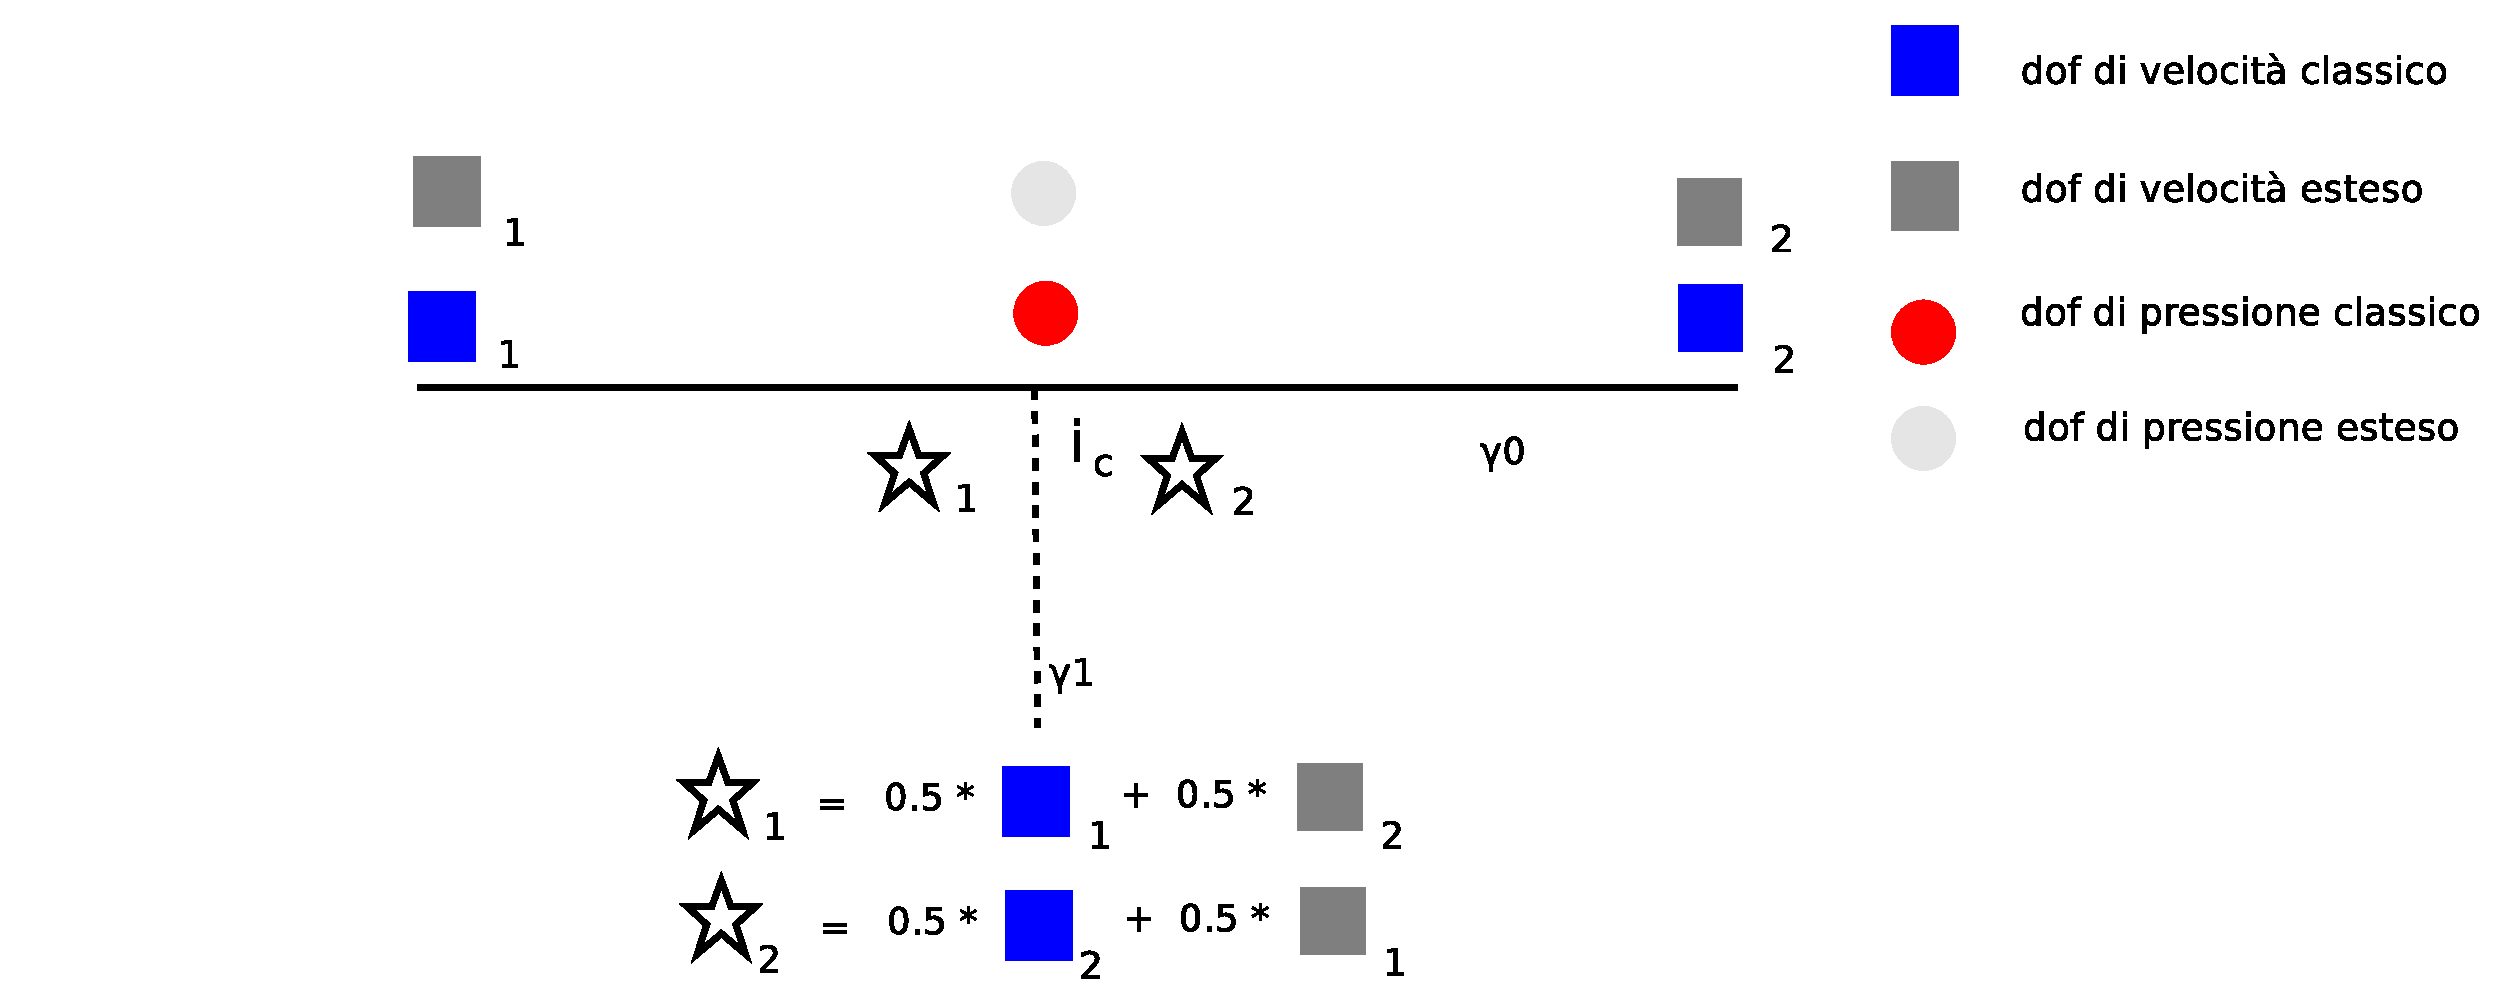
\includegraphics[width=0.8\textwidth]{img/cap6/xfem.eps}
\caption{Introduzione dei gradi di libertà estesi per la frattura tagliata.}\label{xfem}
\end{center}
\end{figure}

\noindent Per quanto riguarda la velocità invece, la velocità prima dell'intersezione lo poniamo par alla media tra il valore nel grado di libertà classico prima e al valore nel grado esteso dopo l'intersezione. Lo stesso facciamo per il valore di velocità dopo l'intersezione, come indicato in figura \ref{xfem}. \\



%\bibliographystyle{plain}
\bibliography{bibliografia}


\bibliographystyle{plain}
\bibliography{bibliografia}

\include{appendice}

\end{document}




\begin{tikzpicture}[remember picture,overlay]
\node [opacity=0.2,scale=0.2] at (current page.center) {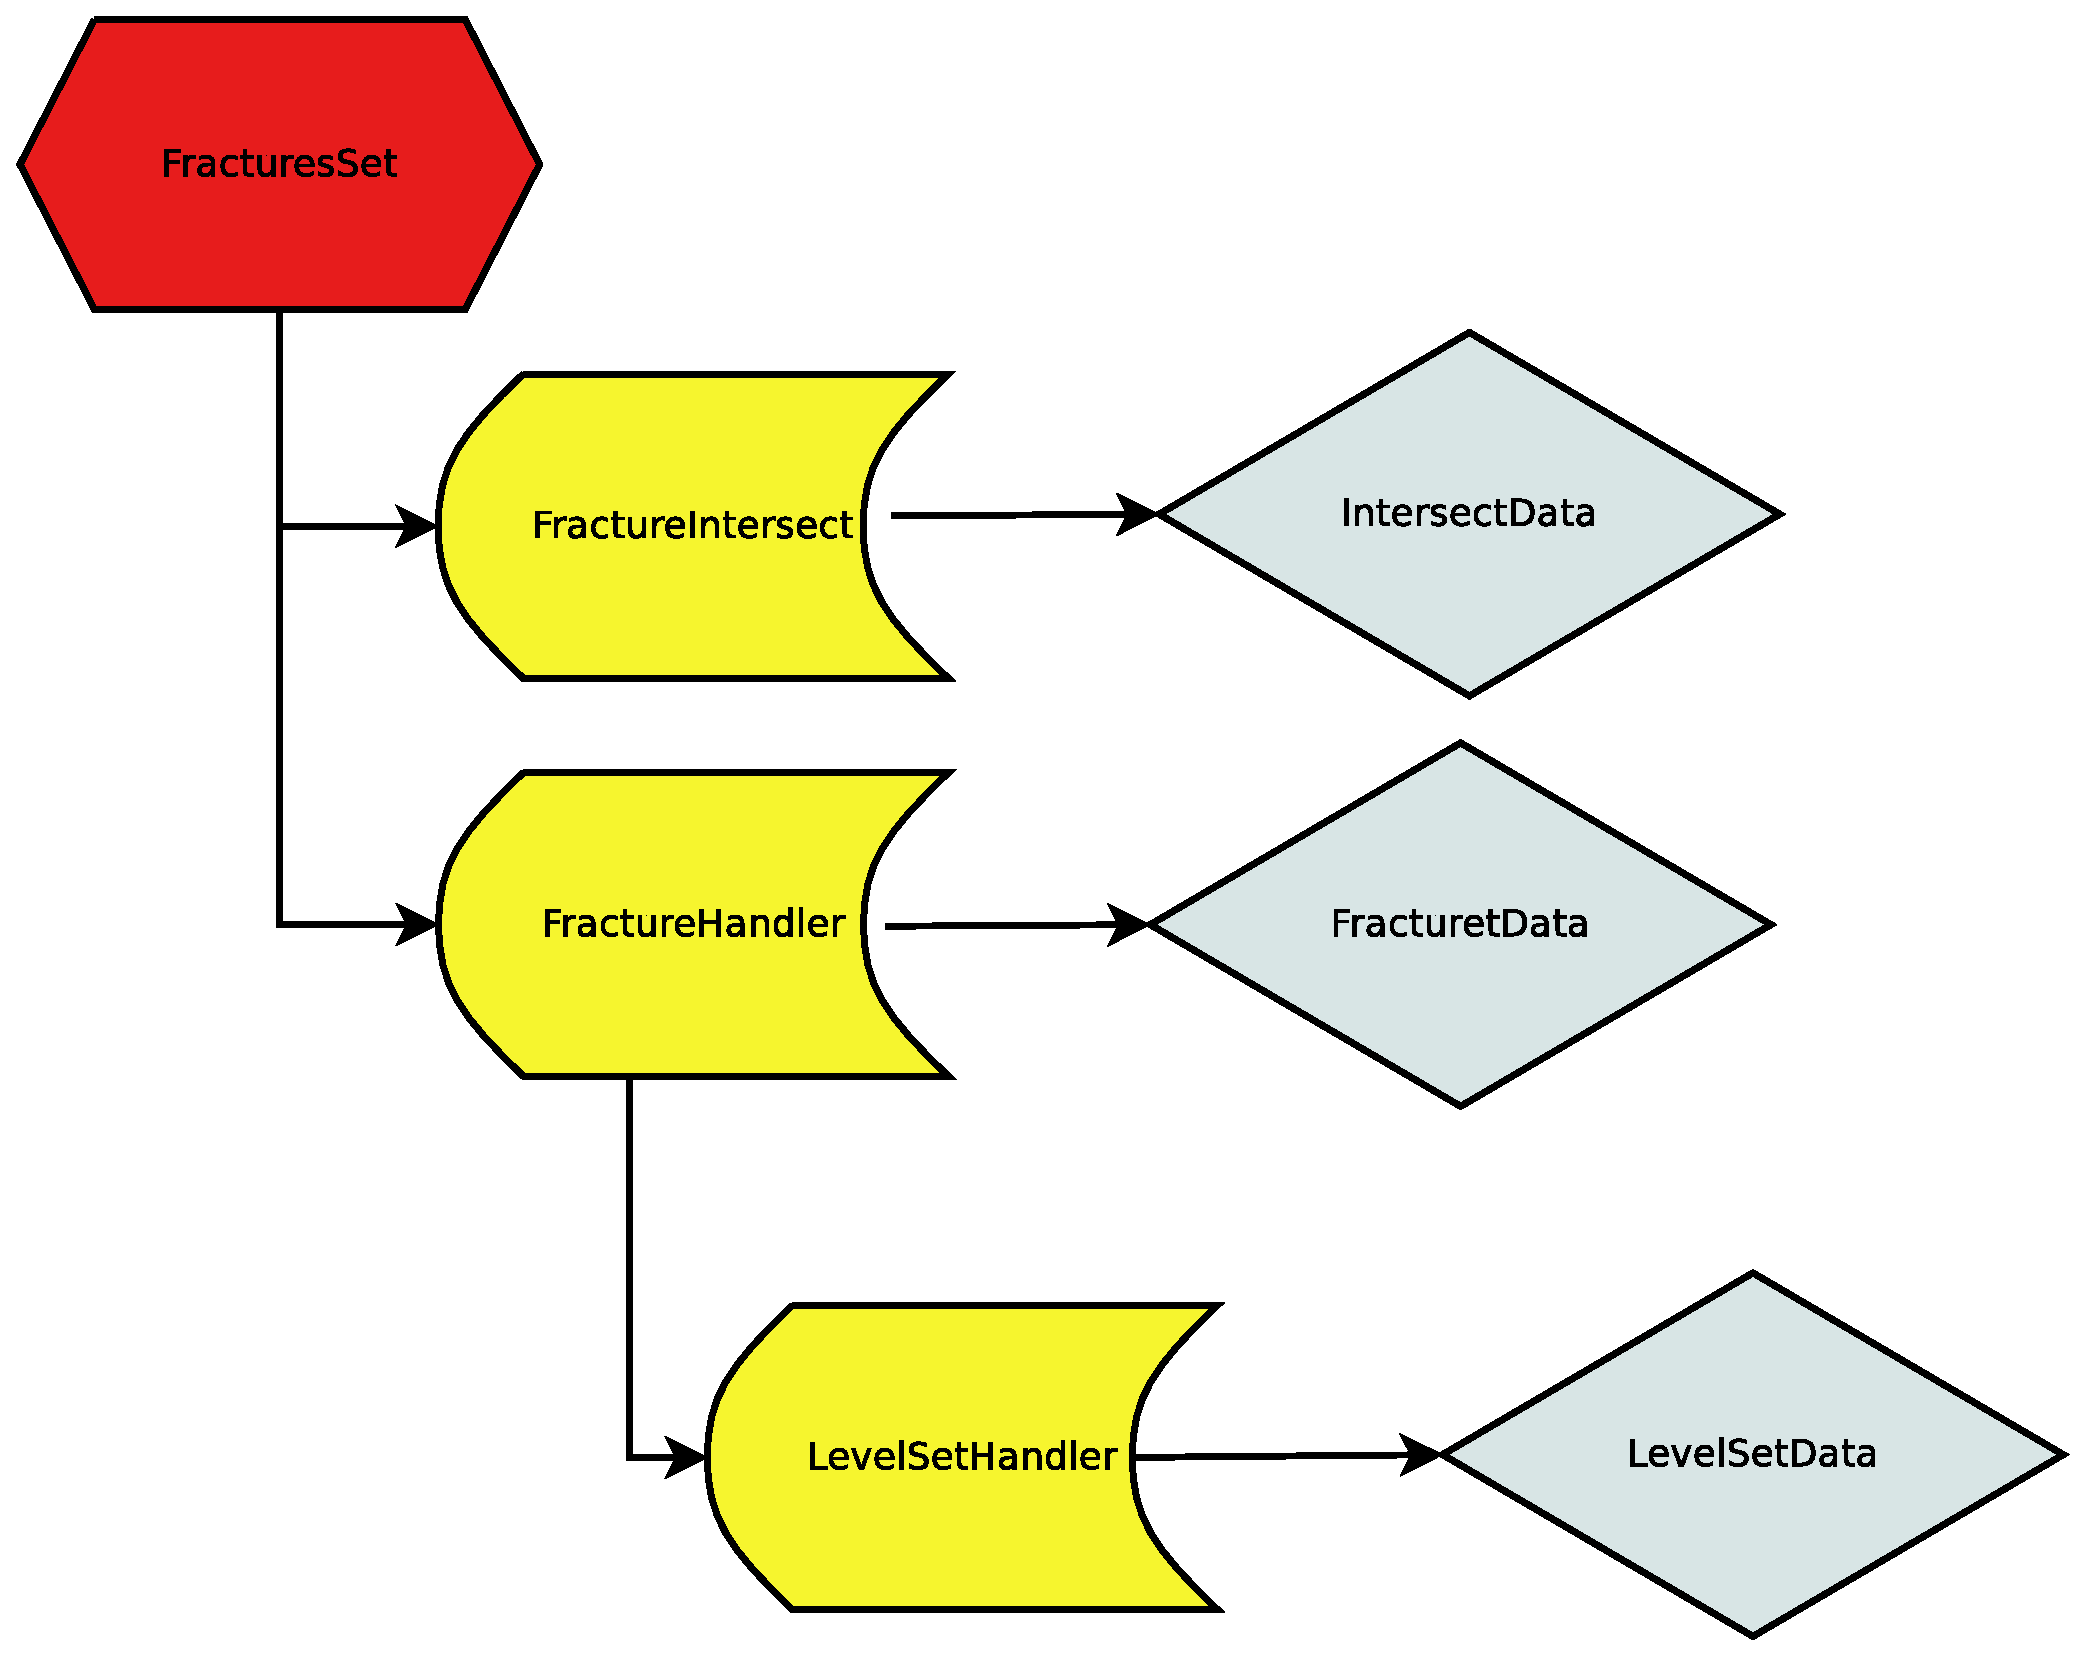
\includegraphics{img/fratture.eps}};
\end{tikzpicture}
